% !TeX program = pdflatex
% !TeX encoding = UTF-8
% !TeX spellcheck = pt_BR
\documentclass[12pt,a4paper]{article}
\usepackage[utf8]{inputenc}
\usepackage[brazil]{babel}
\usepackage{lmodern}			% Usa a fonte Latin Modern
\usepackage{csquotes}			% Aspas e citações mais simples
\usepackage{booktabs}			% Tabelas mais profissionais
\usepackage{placeins}           % Habilita \FloatBarrier, de onde floats não passam!

% Links nas referência cruzada no documento.
% Ajuda a navegação (principalmente no índice).
\usepackage[unicode]{hyperref}
\hypersetup{
    %hidelinks,   % Comente aqui para exibir os links
    colorlinks, % Descomente esse se comentar o de cima
    linkcolor={red!50!black},
    citecolor={blue!50!black},
    urlcolor={blue!80!black}
}

\usepackage[pdftex,dvipsnames,table,xcdraw]{xcolor}

% Melhorias na justificação do texto e
% pequenos ajustes em fontes e alinhamentos. 
\usepackage[T1]{fontenc}
\usepackage{microtype}

% Faz com que linhas orfãs sejam fortemente
% penalizadas. Mas é impossível evitá-las
% completamente.
\clubpenalty=9996
\widowpenalty=9999

% Permite o alinhamento horizontal de várias
% equações, assim elas não tomam muito espaço
% quando são muito pequenas.
\usepackage{tabularx}

% Símbolos diferentes para o texto, como setas →,
% símbolos de copyright e trademark, euro, etc.
% Não é muito útil, mas de vez em quando ajuda.
% Ao invés do comando do latex, dá pra usar o
% caractere em UTF-8 diretamente.
\usepackage{textcomp}

% Pequenos símbolos que são úteis (às vezes)
% como checkmark.
\usepackage{bbding}

% Ajustes finos em comandos do Latex
\usepackage{etoolbox}

% Permite criar formatações específicas, controla
% numerações e produz índices para teoremas e hipóteses.
\usepackage{amsthm}
\usepackage{thmtools}

% Notação de permutação mais 'bonitinha'
\newcommand\Perm[2][^n]{\prescript{#1\mkern-2.5mu}{}P_{#2}}

\declaretheoremstyle[spaceabove=1.5ex,
                     spacebelow=0ex,
                     headindent=\parindent,
                     headformat=\MakeUppercase{\NAME} \NUMBER:\MakeUppercase{\NOTE},
                     notebraces={}{},
                     headpunct=:,
                     bodyfont=\itshape,
                     name=Hipótese]
                     {hypostyle}
\declaretheorem[style=hypostyle]{hypothesis}

% Para listagens de programação ou 
% textos onde a formatação importa
\usepackage{listings}
\lstset{
	inputencoding=utf8,
    extendedchars=true,
	framextopmargin=2pt,
    framexbottommargin=2pt,    
    literate={á}{{\'a}}1
             {ã}{{\~a}}1
             {é}{{\'e}}1
             {í}{{\'i}}1
             {ç}{{\c{c}}}1
             {Ç}{{\c{C}}}1,
}
\renewcommand{\lstlistingname}{Listagem}% Listing -> Listagem
\renewcommand{\lstlistlistingname}{Lista de \lstlistingname s}% List of Listings -> Lista de Listagens

% Permite colocar figuras lado a lado ou
% fazer posicionamentos arbitrários
\usepackage[lofdepth,lotdepth]{subfig}

% Permite o uso da opção "frame" em "includegraphics"
% para fazer uma borda na imagem
\usepackage[export]{adjustbox}

% Para inserir gráficos e imagens
\usepackage{graphicx}
% Diretório padrão para figuras
\graphicspath{ {images/} }

\usepackage{abnt-alf}
\usepackage[top=3cm,bottom=2cm,left=3cm,right=2cm]{geometry}
\usepackage{indentfirst}

% Adiciona o comando \source para citar fontes abaixo
% de figuras. Muito útil!
\usepackage{caption}
\newcommand{\source}[1]{\vspace{-10pt} \caption*{Fonte: {#1}} }

% Facilita o copy 'n paste no PDF
% Remove ligaturas na cópia
\input{glyphtounicode}
\pdfgentounicode=1

% Usado para comentar grandes porções do texto
% com \begin{comment} \end{comment}
\usepackage{comment}

% Para quebrar células de tabelas e melhorar
% a formatação.
% Meio complicado para fazer apenas isso,
% mas funciona.
\usepackage{array}
\usepackage{makecell}

\renewcommand\theadalign{cb}
\renewcommand\theadfont{\bfseries}
\renewcommand\theadgape{\Gape[4pt]}
\renewcommand\cellgape{\Gape[4pt]}

% Texto colorido e afins. Bom para TODO notes
\usepackage{xargs}
\usepackage[normalem]{ulem}
\useunder{\uline}{\ul}{}

% Todo notes.
% Muito útil para deixar anotações enquanto se está
% construindo o texto, depois dá para remover e onde
% quebrar são comentário que devem ser removidos.
% Para remover os comentários do PDF final, basta
% colocar 'disable' na lista de argumentos do pacote:
% \usepackage[disable]{todonotes}
\usepackage[obeyFinal,colorinlistoftodos,prependcaption,textsize=tiny]{todonotes}
\newcommandx{\question}[2][1=]{\todo[linecolor=red,backgroundcolor=red!25,bordercolor=red,#1]{#2}}

\newcommandx{\change}[2][1=]{\todo[linecolor=blue,backgroundcolor=blue!25,bordercolor=blue,#1]{#2}}

\newcommandx{\info}[2][1=]{\todo[linecolor=OliveGreen,backgroundcolor=OliveGreen!25,bordercolor=OliveGreen,#1]{#2}}

\newcommandx{\draft}[2][1=]{\todo[linecolor=Plum,backgroundcolor=Plum!25,bordercolor=Plum,#1]{#2}}

\newcommandx{\thiswillnotshow}[2][1=]{\todo[disable,#1]{#2}}
\reversemarginpar
% END Todo notes.

% Notações matemáticas usadas na dissertação.
% Usando elas é possível trocar toda a notação
% apenas mexendo nesse arquivo. Lembre sempre
% de olhá-lo antes de fazer equações.
% Para fórmulas matemáticas
\usepackage{amsmath}
\usepackage{amssymb}
\usepackage{mathtools}

% Para setas usadas em fórmulas dos grafos
\usepackage{MnSymbol}

% Notações matemáticas usadas com frequência no texto.
% Isso possui três vantagens:
% 1 - Dá menos trabalho digitar as fórmulas
% 2 - Dá mais consistência à notação no trabalho
% 3 - Se mudar de ideia qto à notação, é só trocar aqui
%     e o trabalho todo fica certo.
% Notação matemática
\newcommand{\R}{\mathbb{R}} % Reais
\renewcommand\vec{\mathbf} % vetor como negrito
\newcommand{\avg}[1]{\left\langle #1 \right\rangle} % ... média
\newcommand{\defn}{\coloneqq} % Usamos "=", ":=" ou "\equiv?"
\newcommand{\noloop}[1]{#1^\nlcirclearrowleft} % ... sem loops
% Redes direcionadas
\newcommand{\linkin}[1]{#1^\leftarrow} % ... entrada
\newcommand{\linkout}[1]{#1^\rightarrow} % ... saída
\newcommand{\linkboth}[1]{#1^\leftrightarrow} % ... direcionada
% Redes ponderadas e direcionadas
\newcommand{\win}{w^\leftarrow} % peso e direção de entrada
\newcommand{\wout}{w^\rightarrow} % peso e direção de saída
\newcommand{\weighted}[1]{#1^w} % ... com pesos
\newcommand{\weighteddir}[1]{#1^{w\rightarrow}} % ... com peso e direção
% Reciprocidade
\newcommand{\recin}[1]{#1^\leftlsquigarrow} % ... entrada não-recíproca
\newcommand{\recout}[1]{#1^\leadsto} % ... saída não-recíproca
\newcommand{\recboth}[1]{#1^\leftrightsquigarrow} % ... recíproca
% Capacidades
\newcommand{\capac}{\textit{cap}}

\begin{document}

% CAPA
\pagestyle{empty}
\begin{center}
\large  \textbf{UNIVERSIDADE PRESBITERIANA MACKENZIE}
\large  \textbf{PROGRAMA DE PÓS-GRADUAÇÃO EM}\\
\large  \textbf{ENGENHARIA ELÉTRICA E COMPUTAÇÃO}\\
\vskip 2.0cm
\textbf{\large Ronie Miguel Uliana}\\
\vskip 3.4cm
\setlength{\baselineskip}{1.5\baselineskip}
\textbf{\MakeUppercase{\large Compressão de Fluxo para Identificação de Fronteiras de Carreiras}}\\
\vskip 4.0cm
\end{center}
\hfill{\vbox{\hsize=8.5cm\noindent\strut
Documento de Qualificação apresentado ao \break
Programa de Pós-Graduação em Engenharia \break
Elétrica e Computação da Universidade \break
Presbiteriana Mackenzie como parte dos \break
requisitos para a obtenção do título de \break
mestre em Engenharia Elétrica e Computação.}\\
\strut}
\vskip 3.0cm
\textbf{\normalsize Orientador: Prof. Dr. Leandro Nunes de Castro}\\
\vskip 2.0cm
\begin{center}
São Paulo\\
2017\\
\end{center}

% RESUMO
\newpage
\thispagestyle{plain}
\pagenumbering{roman}
\begin{center}
\large
\textbf{RESUMO}
\end{center}
\renewcommand{\baselinestretch}{0.6666666}
A carreira profissional corresponde à jornada de um indivíduo pelo trabalho, sendo impactada diretamente pela cultura, formação e interesses pessoais. As movimentações de carreira representam passagens entre diferentes trabalhos (por exemplo, empresas ou cargos) e invariavelmente geram expectativas e angústias nos profissionais. A VAGAS.com é uma das principais empresas de recrutamento on-line do Brasil, possuindo o histórico de movimentação de carreira de mais de 10 milhões de brasileiros em mais de 8 mil cargos diferentes. A empresa criou um serviço gratuito, denominado Mapa de Carreiras (MCar), que exibe as principais trajetórias profissionais do mercado obtidas a partir de dados informados nos currículos cadastrados. Esse projeto de pesquisa utiliza uma área do conhecimento que vem se desenvolvendo muito ao longo das duas últimas décadas, denominada Ciência de Redes, para realizar um estudo analítico sobre o MCar. O MCar é uma rede complexa direcionada e ponderada, na qual os nós representam as ocupações profissionais e os arcos indicam a quantidade de profissionais que percorreram o caminho entre cada par de ocupações. Nesse contexto essa dissertação propõe contribuições em duas frentes: 1) proposição de adaptações e derivações de modelos de redes aleatórias existentes para que comportem as características do MCar; e 2) estudos analíticos que permitam compreender ou inferir movimentações profissionais a partir dos dados reais do Mapa de Carreiras.

%%\\[0.5cm]
\begin{flushleft}
{\bf Palavras-chave:} \it{redes, grafos, carreira, ocupações}
\end{flushleft}

% SUMÁRIO
\newpage
\thispagestyle{empty}
\tableofcontents

% DESENVOLVIMENTO
\newpage
\pagestyle{plain}
\pagenumbering{arabic}
\renewcommand{\baselinestretch}{1.5}
\normalsize

\listoftodos[Notas]

%====================================
\section{INTRODUÇÃO}
%====================================

Ao longo da vida profissional é comum para o indivíduo passar por diversas movimentações na carreira. Um estudante de engenharia pode iniciar como Trainee em uma empresa e progredir para Engenheiro, Supervisor de Obras e Diretor de Engenharia. Na área de computação é possível ver um Programador se tornar Analista-Programador, Coordenador de Desenvolvimento, Gerente de Projetos, chegando a Diretor. Esses são casos em que a movimentação de carreira segue um padrão mais tradicional de progressão baseado no plano de carreira de uma organização. Por outro lado, há situações extremas de transições de carreira na qual um Analista-Programador resolve se tornar um Chef de Cozinha ou um Eletricista Industrial passa a atuar como Web Designer. Em qualquer um dos casos, as movimentações de carreira são sempre uma etapa de grande relevância profissional e que, ao mesmo tempo, podem causar estresse, insegurança e alguns desconfortos pelos novos desafios que surgirão.

A movimentação profissional é discutida por modelos como os da \textit{Carreira Proteana} e \textit{Carreira sem Fronteiras}. Esses modelos advogam um distanciamento das carreiras ditadas pelo organograma das empresas em favor de trajetórias com foco maior no indivíduo~\cite{Bendassolli2009-bg}. A Carreira Proteana coloca o indivíduo, e não as organizações, como protagonista da trajetória profissional, onde seus valores são usados na decisão dos próximos passos e o sucesso é subjetivo e medido pela satisfação pessoal~\cite{Hall2004-ke}. A Carreira sem Fronteiras, por sua vez, acontece quando a trajetória se faz independente das organizações ou hierarquias. Essas carreiras são caracterizadas por passagens por múltiplas empresas ou mudanças na especialidade do indivíduo~\cite{Arthur1994-qq}.

No entanto, o movimento de uma pessoa entre ocupações profissionais não é simples. A capacitação do indivíduo, a atratividade da nova ocupação e o próprio conhecimento de que uma transição é possível a tornam mais fácil ou difícil para os profissionais. Quando essa transição é percebida como uma barreira por um número suficiente de pessoas, surge uma \textit{fronteira de carreira}~\cite{Gunz2007-hr}.

Este projeto de pesquisa utiliza o conceito de fronteira de carreira~\cite{Gunz2007-hr}, um banco de dados real com 23 milhões de experiências profissionais~\cite{VAGAS_Tecnologia2014-yv} e técnicas de detecção de comunidades em redes~\cite{Rosvall2009-sd,Edler2017-kt} para encontrar as fronteiras de carreira no mercado de trabalho brasileiro, discutir e entender sua estrutura.

Modelando o problema como um grafo e usando as técnicas de Ciência de Redes, o estudo revela onde estão as fronteiras de carreira e propõe o conceito de \textit{Ilha Ocupacional} para caracterizá-lo. O termo sugere que esses grupos não são formados por alguma característica intrínseca comum entre seus membros, mas sim pelo distanciamento dos outros membros, como proposto por \citeonline{Abbott1995-ft}. Isso significa que as ilhas são uma função da dificuldade da movimentação profissional inter-ilhas e da facilidade de movimentação intra-ilha, independente de atributos derivados de seu conteúdo ou significado.

O estudo prossegue analisando a composição das ilhas e apresenta \textit{insights} sobre sua estrutura. O resultado obtido pode ser usado para o refinamento de teorias sobre carreira, como uma classificação natural para as ocupações baseada na movimentação profissional ou como subsídio para o planejamento de carreiras.

A principal contribuição desse trabalho está em tornar concreto o conceito de \textit{fronteiras de carreira}, revelando a estrutura da movimentação profissional no Brasil. Explorando esse conceito, o trabalho caracteriza a topologia das ilhas ocupacionais e propõe o conceito de \textit{Polos Ocupacionais} como ocupações que possuem papel crucial na estrutura. A topologia encontrada na maior parte das ilhas tende a um formato estrelado, sugerindo que a atuação nos polos afeta a ilha como um todo.

A presença de uma ilha gigante nos resultados fornece indícios que suportam o modelo de \textit{Carreira sem Fronteiras}, ao mesmo tempo em que indica que ela não abrange todos os segmentos profissionais.

Como essa pesquisa é baseada somente nos dados encontrados nos currículos, não é possível responder o que motiva os profissionais nos comportamentos observados, mas independente da motivação, é possível afirmar que o comportamento ocorre. Um estudo dos porquês e das motivações necessita de um aprofundamento psicológico e sociológico que essa pesquisa é incapaz de atingir. Por outro lado, futuros trabalhos nesse sentido podem se apoiar nos resultados aqui obtidos para expandir a compreensão desses comportamentos.

Existem diversas pesquisas sobre movimentação profissional, principalmente sobre os fatores que motivam a mudança, como os expostos por~\citeonline{Ng2007-zp}. Porém, nenhum trabalho pôde ser encontrado analisando redes profissionais sob a ótica da Ciência de Redes, tornado-se outro ponto onde esse trabalho possui contribuições.

Como contribuição final, a movimentação de profissionais é um ponto de interesse para pessoas, empresas e governo. Pessoas desejam saber onde podem chegar, empresas se interessam pela contratação e evolução de seus colaboradores e o setor público traça planos para suprir mão de obra onde ela é insuficiente ou criar oportunidades de trabalho onde ela é abundante. A pesquisa presente traz uma maior compreensão sobre como essa movimentação ocorre e quais sua limitações.

A Seção~\ref{sec:ciencia-de-redes} apresenta as bases teóricas da Ciência de Redes necessárias para esse trabalho. A Seção~\ref{sec:conceitos-sobre-carreiras} discorre sobre os conceitos de carreira. A Seção~\ref{sec:mapa-de-carreiras} descreve os dados e sua transformação em um grafo que representa as transições profissionais no Brasil. A Seção~\ref{sec:fronteiras-de-carreira} combina os dados, conceitos e técnicas apresentado nas seções anteriores para caracterizar a rede, identificar as fronteiras de carreira e analisar a topologia das ilhas resultantes. Finalmente, a Seção~\ref{sec:conclusoes} discorre sobre os resultados encontrados na Seção~\ref{sec:fronteiras-de-carreira} e sugere possíveis usos para eles, bem como novas pesquisas utilizando o mesmo material.

%====================================
\section{CIÊNCIA DE REDES} \label{sec:ciencia-de-redes}
%====================================

A Ciência de Redes (\textit{Network Science}) é uma área de estudo recente. Apesar do estudo matemático de grafos remontar ao século 18, com Leonhard Euler, o estudo de redes tem-se intensificado, culminando em um surto de interesse no começo do século 21 com os trabalhos de Watts-Strogatz e Barabási-Albert~\cite{Watts1998-wt,Barabasi1999-sn} sobre redes complexas.

Redes complexas são grafos com características topológicas que não ocorrem em redes simples ou aleatoriamente geradas, mas que aparecem quando sistemas reais são modelados como grafos, como a conectividade da Internet ou a rede de amigos nas redes sociais~\cite{Barabasi2016-rn}. Uma dessas características é, por exemplo, a presença de \textit{hubs}. Nós com um número anormalmente alto de conexões comparativamente com outros nós da rede.

Um marco para a consolidação da disciplina ocorreu em 2005 com o aval de órgãos governamentais quanto a sua utilidade como ciência. Nesse ano, o exército Norte-Americano solicitou ao \textit{United States National Research Council} um estudo sobre a aplicabilidade da emergente \enquote{Ciência de Redes}. O relatório~\cite{National_Research_Council2006-lv} destaca a relevância do campo em diversas áreas e levanta seus desafios. Nos anos seguintes foram fundados centros de estudos de Ciência de Redes nas universidades norte-americanas com investimentos dos laboratórios de pesquisa do exército~\cite{Maxwell2009-kq}.

O \citeonline{National_Research_Council2006-lv} define a Ciência de Redes como \enquote{o estudo da representação em rede de fenômenos físicos, biológicos e sociais levando a modelos preditivos desses fenômenos}~\footnote{Em tradução livre, \enquote{the study of network representations of physical, biological, and social phenomena leading to predictive models of these phenomena.}}.

Segundo \citeonline{Barabasi2016-rn}, como disciplina, a Ciência de Redes se diferencia de uma abordagem tradicional pelos seguintes pontos:

\begin{description} \label{desc:ciencia-de-redes}
	\item[\textit{Interdisciplinar}.] A Ciência de Redes é terreno comum para diversas disciplinas, como Biologia (com redes de proteínas), Sociologia (com redes sociais), Computação (com redes de comunicações e algoritmos), entre outras. Apesar de divergirem em essência e propósito, as redes que são seu objeto de estudo compartilham características e propriedades.
    
    \item[\textit{Empírica}.] A Ciência de Redes foca em dados reais e no propósito de uso das redes. Modelos teóricos são confrontados com dados reais para avaliação de sua utilidade na descoberta de propriedades relevantes das redes.
    
    \item[\textit{Matemática e Quantitativa}.] A Ciência de Redes baseia-se fortemente na Teoria de Grafos, na Estatística e em Algoritmos para criação de modelos e sua avaliação. A descoberta de princípios gerais de organização das redes só é possível com uma sólida base formal Matemática.
    
    \item[\textit{Computacional}.] Redes reais por vezes são de grande tamanho, com milhares ou milhões de nós, como a Internet ou as relações entre trabalho e pessoas. As características de algumas topologias, como a distribuição dos graus dos nós, somente são distinguíveis quando o número de nós e conexões é bastante grande. Adicionalmente, as análises comparativas com modelos nulos pressupõe a geração de grandes quantidades de redes aleatórias de composição similar às redes em estudo, um trabalho que não é possível sem o uso intensivo de computadores. Algoritmos e técnicas de processamentos de grandes volumes de dados são ferramentas essenciais para esses estudos.
\end{description}

%====================================
\subsection{Conceitos de Redes}

É preciso descrever os conceitos utilizados em redes para compreensão desse trabalho. Apesar de serem básicos em Teoria de Grafos, uma breve descrição é oferecida nas seções seguintes para completude dessa obra.

Um \textit{grafo} ou \textit{rede} é uma abstração usada quando o foco do estudo está no relacionamentos entre entidades. Nessa abstração, outras características das entidades que não o relacionamento são descartadas. Redes são representadas graficamente por formas geométricas, em geral pequenos círculos para representar as entidades, conectados por linhas representando os relacionamentos (Figura~\ref{fig:exemplo-tipos-grafo}).

\begin{figure}[ht]
    \centering
    \subfloat[][simples] {
        \includegraphics[scale=0.5]{simple.pdf}
        \label{fig:exemplo-grafo-simples}
    }
    \subfloat[][direcionado] {
        \includegraphics[scale=0.5]{directed.pdf}
        \label{fig:exemplo-grafo-direcionado}
    }    
    \subfloat[][ponderado] {
        \includegraphics[scale=0.44]{weighted.pdf}
        \label{fig:exemplo-grafo-ponderado}
    }    
    \caption{Redes ou Grafos}
    \label{fig:exemplo-tipos-grafo}
    \source{Elaboração do autor}
\end{figure}

As entidades da rede são chamadas \textit{nós} ou \textit{vértices}, enquanto os relacionamentos são chamados \textit{conexões} ou \textit{arestas}. Os artigos científicos sobre Ciência de Redes dão preferência aos termos \textit{rede}, \textit{nó} e \textit{conexão}, enquanto no campo da Teoria de Grafos os termos são \textit{grafo}, \textit{vértice} e \textit{aresta}~\cite[p.~45]{Barabasi2016-rn}. Nesse trabalho deu-se preferência pelos termos usados em Ciência de Redes, no entanto, os termos de Teoria de Redes, quando usados, são considerados sinônimos.

Quando os relacionamentos possuem uma certa direção eles formam \textit{redes direcionadas} (Figura~\ref{fig:exemplo-grafo-direcionado}). Por exemplo, uma rede que representa as trocas de presentes natalinos é uma rede em que há \textit{direção}, o presente é dado de uma pessoa \textit{para} outra. Em outros casos, quando não há uma direção no relacionamento, a rede é chamada \textit{não-direcionada}. Por exemplo, em uma rede de relacionamentos os indivíduos se conhecem mutuamente. Uma conexão direcionada é por vezes chamada \textit{arco}.

Se a intensidade do relacionamento é relevante as conexões ganham um \textit{peso} (Figura~\ref{fig:exemplo-grafo-ponderado}). Seu significado depende da rede em questão. Por exemplo, em uma rede de transportes o peso pode significar a distância entre locais de entrega, em uma rede de dados pode significar o volume do tráfego entre os pontos, e em uma rede social pode significar o número de mensagens trocadas entre duas pessoas. Redes onde existe a presença de conexões com peso são chamadas \textit{redes ponderadas}.

Algumas redes permitem múltiplas conexões entre dois nós (Figura~\ref{fig:exemplo-grafo-multiplo}). Por exemplo, em uma rede de ligações telefônicas é possível representar cada ligação por uma conexão diferente, duas pessoas que troquem ligações seriam representadas por dois nós com diversas conexões entre si, uma para cada ligação feita. Redes que permitem múltiplas conexões são chamadas \textit{multigrafos}. Dependendo do fenômeno sendo modelado, multigrafos podem ser representados por redes ponderadas, em especial redes onde o relacionamento significa fluxo~\cite{Newman2004-by}.

\begin{figure}[ht]
    \centering
    \subfloat[][laços e direção] {
        \includegraphics[scale=0.5]{loop.pdf}
        \label{fig:exemplo-grafo-laco}
    }
    \subfloat[][múltiplas conexões] {
        \includegraphics[scale=0.5]{multiple.pdf}
        \label{fig:exemplo-grafo-multiplo}
    }    
    \caption{Redes com laços e conexões múltiplas}
    \source{Elaboração do autor}
\end{figure}

Em algumas redes, não há sentido em nós que conectam a si mesmos, por exemplo, em uma rede social onde as conexões representam quem conhece quem, uma conexão de alguém consigo mesmo não é relevante para o estudo da rede (desconsiderando-se questões filosóficas). Já em outras redes é natural considerar esse tipo de conexão, como uma que modele a transição de estados de uma máquina em que uma ação pode resultar na permanência no mesmo estado. Conexões de um nó com ele mesmo são chamados \textit{laços} ou \textit{loops} (Figura~\ref{fig:exemplo-grafo-laco}).

Redes que não permitem laços, pesos ou conexões múltiplas são chamadas \textit{redes simples} (Figura~\ref{fig:exemplo-grafo-simples}).

% Ronie: Mover o parágrafo abaixo para a seção do Mapa de Carreiras?
Nessa pesquisa, o problema foi modelado como uma rede direcionada, ponderada e com laços. Cada ocupação é um nó, a movimentação de profissionais entre as ocupações são conexões direcionadas e ponderadas e os profissionais que permanecem na mesma ocupação mas mudam de empresa são modelados como laços.

O conceito de \textit{componente} é importante para esse trabalho e está relacionado a partes da rede que estão desconectadas entre si. Se existirem nós em uma rede que estão conectados entre si, mas não se conectam a nenhum outro nó, então essa rede \enquote{isolada} é um \textit{componente}. Um nó sem conexões pode ser considerado um componente de tamanho~1. Uma rede em que todos os nós se conectam de maneira direta ou indireta é chamada de \textit{rede conectada} e possui apenas um componente. Um componente é um subgrafo em que todos os seus nós possuem conexão direta ou indireta entre si, porém nenhum de seus nós se conecta ao resto da rede. Uma exemplo de rede com três componentes pode ser observado na Figura~\ref{fig:exemplo-componente}.

\begin{figure}[ht]
    \centering
    \includegraphics[scale=0.7]{componente.png}
    \caption{Rede com três componentes}
    \source{Wikimedia - David Eppstein}
    \label{fig:exemplo-componente}
\end{figure}

Em algumas topologias de rede surgem nós com um número de conexões muito acima do esperado, chamados \textit{hubs}. O número de conexões de um nó é chamado de \textit{grau} do nó, portanto, \textit{hubs} são nós de alto grau. Esse é um conceito central no estudo de redes complexas por não aparecerem em redes aleatórias, mas figurarem em diversas redes reais.

No estudo de redes, os nós de maior importância são considerados nós centrais da rede. Como é responsabilidade de cada estudo definir o que é \textit{importante}, existem várias medidas de centralidade, indo desde a simples contagem de nós com mais conexões (centralidade de grau) até a medição de nós que participam de fluxos de maior volume.

A \textit{Centralidade de Grau} identifica os nós que mais se relacionam diretamente com o resto da rede. Dada sua conectividade, os nós com maior centralidade de grau encurtam os caminhos na rede, uma vez que conectam uma maior quantidade de nós entre si através de um único \enquote{salto}. Esses mesmos nós criam rapidamente novos caminhos possíveis na rede conforme seu grau aumenta, um nós de grau 2 possui apenas 2 caminhos possíveis passando por ele (ida e volta), enquanto um nó de grau 3 possui 6 caminhos possíveis e um nó de grau 4 possui 12 caminhos possíveis. Mais precisamente, o número de caminhos possíveis $P^*$ passando por um nó é uma permutação do grau $k$ do nó tomados 2 a 2 na forma

\begin{equation*}
P^*(k) = \Perm[k]{2} = \frac{k!}{(k - 2)!}\,.
\end{equation*}

Em uma rede direcionada, por outro lado, o número de caminhos possíveis que passa por um nó é uma simples multiplicação entre o grau de entrada $k^\leftarrow$ pelo grau de saída $k^\rightarrow$, $P^*(k) = k^\leftarrow k^\rightarrow$.

A \textit{Centralidade de Fluxo}~\cite{Freeman1991-on} existe apenas em redes que as conexões representam a movimentação entre entidades, portanto, apenas para redes ponderadas e direcionadas. Nós com maior centralidade são os nós por onde a maior parte do fluxo passa, uma perturbação nesses nós influencia...

(EXPANDIR...)

A medida de \textit{Assortatividade} significa que nós que compartilham características comuns tendem a se conectar com mais frequência. \textit{Desassortatividade} é o conceito contrário, onde nós com características diferentes tendem a se conectar mais frequentemente. Na Ciência de Redes é comum o termo ser associado a tendência de nós de mesmo grau se conectarem entre si. A assortatividade é detalhada na Seção~\ref{sec:assortatividade}. A grosso modo, uma assortatividade de grau negativa significa que a topologia da rede se assemelha à estrutura de \enquote{centro e raios\footnote{Em inglês: \enquote{Hub and Spokes}}}. Esse medida é importante na caracterização das ilhas ocupacionais.

(EXPANDIR) Bigramas e Trigramas

(EXPANDIR) Source e Sink

%====================================
\subsubsection{Redes Multicamadas} \label{sec:multicamadas}

Redes reais nem sempre podem ser modeladas como redes simples. Múltiplos tipos de relacionamentos como comunicação por email, telefone e pessoalmente; diferentes tipos de nós, como humanos e máquinas ou ainda diferentes momentos de interação, como conversas em um evento, bar ou no trabalho são características importantes que não são facilmente modeladas por redes tradicionais~\cite{Kivela2014-pb}.

Ao longo das últimas décadas, variações de modelos de rede foram utilizadas para modelar esses fenômenos, como redes multiplexadas, redes multirrelacionais e \enquote{redes de redes}. Em seu trabalho, \citeonline{Kivela2014-pb} propõem uma padronização dessas definições ao redor do termo Redes Multicamadas.

Uma rede multicamada representa a diversidade de nós e conexões acima exemplificados como uma rede em os nós possuem múltiplas representações, cada uma em uma \textit{camada} diferente. Um exemplo de rede multicamada pode ser visto na Figura~\ref{fig:ex-multicamada}.

\begin{figure}[ht]
    \centering
    \includegraphics[scale=0.4]{random_walks_on_multilayer_networks}
    \caption{Exemplo do caminhar de um \textit{random walker} em uma rede multicamada.}
    \source{Wikimedia - Manlio De Domenico}
    \label{fig:ex-multicamada}
\end{figure}

Nessa trabalho, a rede multicamada é usada para simplificar uma rede modelada como um processo de Markov de segundo nível. Essa simplificação permite traduzir a Equação de Mapa (apresentada mais à frente, na Seção~\ref{sec:infomap}) para detectar sobreposições entre comunidades, ou seja, comunidades que compartilham nós.

%====================================
\subsection{Medidas de Rede} \label{sec:medidas-de-rede}

As medidas descritas nessa seção são usadas para caracterização da rede do MCar bem como das ilhas ocupacionais encontradas.

Entenda-se por \textit{caracterização} a descrição da rede utilizando medidas numéricas que permitam a interpretação dos macro-atributos da rede. Por exemplo, a medida de assortatividade é usada para identificar que a topologia predominante nas ilhas ocupacionais se assemelha a de \textit{centro e raios}, enquanto a medida de centralidade de fluxo e de grau são usadas para identificar as ocupações mais importantes nas ilhas.

%===================================
\subsubsection{Assortatividade} \label{sec:assortatividade}

A assortatividade é uma medida de quão nós similares estão conectados entre si~\cite{Newman2003-jn}. Quaisquer atributos dos nós podem ser usados como medida de assortatividade, por exemplo, se nós representarem pessoas e as conexões representarem amizades, medir a assortatividade de idade diria se as pessoas preferem amizades com outras de idade similar (assortatividade positiva) ou preferem amizades com pessoas muito mais velhas ou novas (assortatividade negativa ou desassortatividade).

A assortatividade de grau é de especial interesse na análise de redes, pois permite caracterizar sua topologia. Redes com assortatividade negativa (desassortativas), remetem à topologia de \textit{eixo e raios} ou \textit{estrela}, onde nós de grau muito alto (\textit{hubs}) se conectam a muitos nós de grau mais baixo~\cite{Barabasi2016-rn}. A Figura~\ref{fig:assortatividade-topologia} mostra um exemplo de uma rede em que predomina essa topologia.

Quanto menor a assortatividade, mais a rede se aproxima da topologia de estrela, em que todos os nós de alto grau conectam-se somente a nós de grau muito baixo. Como exemplos, a ilha ocupacional relacionada a \enquote{Fonoaudiologia} na Figura~\ref{fig:ex-assortatividade-negativa}, com assortatividade $-0,99$, possui todos os nós conectados a um \textit{hub} central, com nenhuma conexão entre as ocupações periféricas. Já a ilha relacionada a \enquote{Coordenador de Mídia} na Figura~\ref{fig:ex-assortatividade-positiva}, com assortatividade $0,18$, possui uma estrutura um pouco mais distribuída e o grau dos nós é similar, com exceção do próprio \enquote{Coordenador de Mídia}.

\begin{figure}[ht]
    \centering
    \subfloat[][Assortatividade $-0,99$] {
        \includegraphics[width=0.4\linewidth]{ex-assortatividade-negativa.pdf}
        \label{fig:ex-assortatividade-negativa}
    }
    \subfloat[][Assortatividade $0,18$] {
        \includegraphics[width=0.4\linewidth]{ex-assortatividade-positiva.pdf}
        \label{fig:ex-assortatividade-positiva}
    }    
    \caption{Assortatividade e Topologia}
    \label{fig:assortatividade-topologia}
\end{figure}

A assortatividade de grau em uma rede direcionada pode ser caracterizada pelo coeficiente de correlação de Pearson dos graus~\cite{Barabasi2016-rn}. Seja $k_i^\leftarrow$ e $k_i^\rightarrow$,  respectivamente, os graus de entrada e saída do nó $i$, seja $E$ o conjunto de conexões da rede, $e = (m, n) \mid e \in E$ as conexões de $E$, $m$ o vértice de onde $e$ sai e $n$ o vértice para onde $e$ aponta, definem-se os \textit{graus remanescentes} de entrada e saída, respectivamente, $\delta_e^\leftarrow$ e $\delta_e^\rightarrow$ da conexão $e$ como
\begin{align*}
\delta_e^\leftarrow &= k_n^\leftarrow - 1
\\
\delta_e^\rightarrow &= k_m^\rightarrow - 1\,.
\end{align*}

\begin{figure}[ht]
    \centering
    \includegraphics[scale=0.4]{remaining-degree.pdf}
    \caption{Graus remanescentes de entrada e saída da conexão $e$}
    \label{fig:remaining-degree}
\end{figure}

O \textit{grau remanescente} é o grau do nó, excetuando-se a conexão atual (Figura~\ref{fig:remaining-degree}). A correlação de Pearson $r$ dos graus é então definida por

\begin{align*}
p &= \sum_{e \in E} \delta_e^\leftarrow \delta_e^\rightarrow
\\
q &= \frac{1}{|E|} \sum_{e \in E} \delta_e^\leftarrow
\sum_{e \in E }\delta_e^\rightarrow
\\
\sigma^2_\leftarrow &= \sum_{e \in E} \left( \delta_e^\leftarrow \right)^2
- \frac{1}{|E|} \left( \sum_{e \in E} \delta_e^\leftarrow \right)^2
\\
\sigma^2_\rightarrow &= \sum_{e \in E} \left( \delta_e^\rightarrow \right)^2
- \frac{1}{|E|} \left( \sum_{e \in E} \delta_e^\rightarrow \right)^2
\\
r &= \frac{p - q}
{\sqrt{ \sigma^2_\leftarrow } \sqrt{ \sigma^2_\rightarrow }}\,.
\end{align*}

%====================================
\subsubsection{Coeficiente de Agrupamento} \label{sec:coeficiente-agrupamento}

O \textit{coeficiente de agrupamento local} é a medida de quanto os vizinhos de um nó estão conectados entre si e é dado por:

\begin{equation}
c_c(i) \defn \begin{cases}
    \frac{2m_i}{k_i(k_i - 1)} & \text{se}\ k_i > 1 \\
    \text{indefinido}         & \text{caso contrário}
  \end{cases}
\end{equation}

Onde $m_i$ é o número de conexões entre os vizinhos do nó $i$, e $k_i$ é o número de conexões de $i$.

O coeficiente de agrupamento local pode ser estendido para grafos direcionados distinguindo-se a direção da conexão.

\begin{equation}
\linkboth{c}_c(i) \defn \begin{cases}
    \frac{\linkboth{m}_i}{k_i(k_i - 1)} & \text{se}\ k_i > 1 \\
    \text{indefinido}                  & \text{caso contrário}
  \end{cases}
\end{equation}

Onde $\linkboth{m}_i$ é o número de conexões entre os vizinhos de $i$.

Em um grafo ponderado, \citeonline{Barrat2004-xf} oferecem a seguinte versão do coeficiente de agrupamento:

\begin{equation}
\weighted{c}_c(i) \defn \frac{1}{s_i(k_i - 1)} \sum_{j,k \in N(i)} \frac{w_{ij} + w_{jk}}{2}
\end{equation}

Onde $N(i)$ é o conjunto de vizinhos de $i$, $w_{ij}$ é o peso da conexão entre os nós $i$ e $j$ e $s(i)$ é a força do nó.

O \textit{coeficiente de agrupamento global} de um grafo é dado pela média dos coeficientes locais:

\begin{equation}
C_c \defn \frac{1}{|N'|} \sum_{i \in N'} c_c(i)
\end{equation}

Onde $N'$ é o conjunto de nós com grau maior que 1, ou seja, $N' = \left\lbrace i \in N \mid k_i > 1 \right\rbrace$. O coeficiente de agrupamento para um grafo ponderado é calculado da mesma forma, apenas substituindo-se o coeficiente local por sua versão ponderada.

\begin{comment}
%====================================
\subsubsection{Similaridade} \label{sec:similaridade}

A \textit{similaridade} é usada para medir se dois nós ou conexões são similares estruturalmente, ou seja, independente do seu conteúdo. De maneira simplificada, dois nós são tão mais similares quanto houverem vizinhos comuns. Já a \textit{similaridade de conexão}, como definida por \citeonline{Ahn2010-uh}, parte de conexões que compartilham um nó e verifica se os nós não compartilhados são similares.

A similaridade também é usada como medida de distância em algoritmos de agrupamento hierárquico \cite{Barabasi2016-rn}.

Existem diversas formulações para a similaridade e \citeonline{Lu2011-og} revisam dez delas sem considerar suas variações para redes direcionadas e ponderadas. Esse trabalho utiliza a similaridade baseada no índice de Jaccard (Equação~\ref{eq:similaridade-1}) e suas variações.

Sejam $i$ e $j$ nós da rede, $N_i$ o conjunto de vizinhos do nó $i$ e $N_i^+ \defn N_i \cup \{i\}$, a Equação~\ref{eq:similaridade-1} define a similaridade por vizinhança e a Equação~\ref{eq:similaridade-2} define a mesma similaridade considerando a existência de conexão direta entre os nós sendo comparados.

\noindent
\begin{tabularx}{\linewidth}{@{}XX@{}}
    \begin{equation} \label{eq:similaridade-1}
        S_{ij} \defn \frac{|N_i \cap N_j|}{|N_i \cup N_j|} 
    \end{equation} &
    \begin{equation} \label{eq:similaridade-2}
        S_{ij}^+ \defn \frac{|N_i^+ \cap N_j^+|}{|N_i^+ \cup N_j^+|} 
    \end{equation}
\end{tabularx}

Em redes direcionadas é preciso distinguir os vizinhos de entrada e saída. A similaridade em uma rede direcionada $\linkboth{S}_{ij}$ é dada pela média entre similaridade de entrada e saída (Equação~\ref{eq:similaridade-3}).

\begin{equation} \label{eq:similaridade-3}
    \linkboth{S}_{ij} \defn \frac{1}{2} \left( \frac{|\linkin{N}_i \cap \linkin{N}_j|}{|\linkin{N}_i \cup \linkin{N}_j|} + \frac{|\linkout{N}_i \cap \linkout{N}_j|}{|\linkout{N}_i \cup \linkout{N}_j|} \right)
\end{equation}

Onde $\linkin{N}_i$ é o número vizinhos de $i$ em que as conexões chegam a ele e $\linkout{N}_i$ é o número de vizinhos onde a conexão parte de $i$.

No caso de redes ponderadas e direcionadas, o índice de Jaccard pode ser generalizado no coeficiente de Tanimoto, resultando na similaridade $\weighteddir{S}_{ij}$ da Equação~\ref{eq:similaridade-3} \cite{Ahn2010-uh}. Sendo $W$ a matriz de pesos da rede e $w_{ij}$ o peso da conexão direcionada de $i$ a $j$, define-se o vetor $\vec{w}_i = (w_{i1},w_{i2},\ldots,w_{in})$ como sendo o vetor de pesos das conexões do nó $i$, onde $n$ é o número de nós da rede e $w_{ij} = 0$ se não há conexão entre os nós.

\begin{equation}
\weighteddir{S}_{ij} \defn \frac{\vec{w_i} \cdot \vec{w_j}}{|\vec{w_i}|^2 + |\vec{w_j}|^2 - \vec{w_i} \cdot \vec{w_j}}
\end{equation}

Para o agrupamento de conexões, como proposto por \citeonline{Evans2009-lq} e \citeonline{Ahn2010-uh}, é preciso definir a similaridade entre conexões. Sendo o vetor $\vec{r}_{i} \defn (r_{i1}, r_{i2}, \ldots, r_{iN})$ definido de acordo com a Equação~\ref{eq:similaridade-conexao-parcial}:

\begin{equation} \label{eq:similaridade-conexao-parcial}
r_{ij} \defn \frac{1}{k_i} \sum_{h \in N_i} w_{ih}\delta_{ij} + w_{ij}
\end{equation}

Onde $\delta_{ij} = 1$ se $i = j$ e zero caso contrário. A similaridade entre conexões $R_{(i,h),(h,j)}$ pode ser definida como \cite{Ahn2010-uh}:

\begin{equation}
R_{(i,h),(j,h)} \defn \frac{\vec{r_i} \cdot \vec{r_j}}{|\vec{r_i}|^2 + |\vec{r_j}|^2 -  \vec{r_i} \cdot \vec{r_j}}
\end{equation}

Onde $(i,h)$ e $(j,h)$ são as conexões que compartilham o nó $h$ e $i \neq h \neq j$. O nó compartilhado não é usado no cálculo da similaridade, mas é pré-requisito para considerar que duas conexões são similares. A similaridade de conexão é usada principalmente na detecção de comunidades.
\end{comment}

%====================================
\subsubsection{Modularidade} \label{sec:modularidade}

\question[inline]{Passar essa seção para dentro de detecção de comunidade?}

A \textit{modularidade} é uma medida de qualidade para a detecção de comunidades. O algoritmo de Louvain~\cite{Blondel2008-qh}, por exemplo, usa a modularidade como função objetivo. De certa forma ela tem uma relação com o coeficiente de agrupamento, no sentido que ambas procuram quantificar o quanto nós estão mais densamente conectados que outros.

Essa medida é aplicada apenas a um grafo que foi particionado em comunidades. Em termos gerais, ela indica se um grupo de nós é mais densamente conectado que o esperado em uma rede aleatória com o mesmo número de nós e conexões, em caso afirmativo, esse conjunto é uma possível comunidade. Para o caso em que ela reflete um comportamento próximo do que seria esperado em uma rede aleatória, não é possível afirmar que esse grupo tenha qualquer característica especial que o transforme em uma comunidade. No caso de modularidade negativa, isto é, em que a densidade de conexões é menor do que o esperado, esse grupo não representa uma comunidade~\cite{Barabasi2016-rn}.

A modularidade $m_c$ de um grupo $c$ de nós pode ser definida como:

\begin{equation} \label{eq:modularidade-local}
m_c \defn \frac{L_c}{L} - \left( \frac{K_c}{K} \right)^2
\end{equation}

Onde $L$ é o número total de conexões da rede, $K = 2L$ é a soma de todos os seus graus, $L_c$ é o número de conexões do grupo e $K_c$ é a soma de seus graus.

Assumindo que uma rede foi particionada em $N_c$ grupos, a modularidade total $M_c$ pode ser calculada somando-se a modularidade de cada grupo:

\begin{equation} \label{eq:modularidade-global}
M_c \defn \sum_{c \in N_c} m_c
\end{equation}

O uso da modularidade para detecção de comunidades possui a limitação que o maior valor possível da modularidade $M_\textit{max}$ possui a tendência de formar um platô, dificultando a detecção da partição ótima~\cite{Barabasi2016-rn}.

Considerando as Equações \ref{eq:modularidade-local} e \ref{eq:modularidade-global}, quando dois grupos $A$ e $B$ são unidos, a diferença esperada em $M_c$ é:

\begin{equation}
\Delta M_{AB} \defn \frac{l_{AB}}{L} - \frac{k_A k_B}{2L^2}
\end{equation}

Onde $l_{AB}$ é o número de conexões que conectam os dois grupos, e $k_A$ e $k_B$ são as somas de graus de $A$ e $B$, respectivamente. Quando $\frac{k_A k_B}{2L^2} < \frac{l_{AB}}{L}$, a modularidade aumenta ($\Delta M_{AB} > 0$) se houver ao menos uma conexão entre os grupos ($l_{AB} \geq 1$). Isso significa que esses grupos unidos aumentam a modularidade, mesmo sendo grupos diferentes. Esse efeito é chamado de \textit{limite de resolução}.

É possível observar que a resolução da modularidade é diretamente proporcional ao número total de conexões da rede. Diminuindo-se o número de conexões, $k_A$ e $k_B$ se tornam mais relevantes que $l_{AB} / L$. Portanto, para contornar essa limitação é possível considerar os maiores grupos da partição como uma única rede e reparticioná-la. Dessa forma, os grupos artificialmente unidos por conta da resolução serão separados.


%====================================
\subsection{Detecção de Comunidade} \label{sec:deteccao-comunidade}

Detecção de Comunidade, Particionamento de Grafo ou Agrupamento (\textit{Clustering}) são nomes equivalentes para a atividade de se encontrar conjuntos de nós que possuem ligações mais fortes entre si do que com o resto da rede.

Uma \textit{comunidade} é um subgrafo com conexões mais \textit{coesas} entre seus nós do que com o restante do grafo. A palavra \enquote{coesão} aqui pode ser interpretada de várias maneiras. Para \citeonline{Ahn2010-uh,Evans2009-lq}, uma comunidade é definida quando o número de conexões internas do subgrafo é maior que o número de conexões que o conecta ao resto do grafo. Para \citeonline{Barabasi2016-rn,Newman2004-jg} a comunidade deve possuir uma densidade de conexões mais alta do que o esperado em uma rede aleatória equivalente. Para esses autores, o número de conexões é o fator determinante para a identificação da comunidade.

\citeonline{Rosvall2009-sd} e \citeonline{Van_Dongen2000-qm}, por sua vez, trabalham a detecção de comunidades como a identificação de fluxos mais frequentes na rede. Assumindo que uma conexão representa um fluxo, \textit{coesão} significa que comunidades possuem fluxo maior entre seus nós do que com outros fora da comunidade.

Essas abordagens distintas são aplicáveis a cenários diferentes. A densidade de conexões é mais adequada em redes onde a estrutura é importante, como, por exemplo, em uma rede social. Já em redes que representam fluxos, como circuitos ou redes de transporte, a segunda abordagem é mais atraente~\cite{Rosvall2009-sd}.

Na visão de \citeonline{Barabasi2016-rn} a detecção de comunidade se apoia em quatro hipóteses. Contrastar essas hipóteses com os conceitos de \citeonline{Rosvall2009-sd} destaca a diferença entre as abordagens e torna mais claras as situações onde são mais adequadamente aplicadas.

\begin{description}
%--------------------------------
\item [Hipótese Fundamental] \textit{A estrutura de comunidade de uma rede é codificada unicamente em seu diagrama de conexões.}

Isso significa que não é possível identificar comunidades somente pelos seus graus, nós ou quaisquer medidas que não envolvam a estrutura de conexão da rede. A detecção de comunidades só é possível analisando-se a conectividade entre os nós, seja através de uma matriz de adjacência ou outro artefato que permita a investigação das conexões.

Essa hipótese é válida em qualquer uma nas definições detecção de comunidades mencionadas no início dessa Seção.

%--------------------------------
\item [Hipótese da Conectividade e Densidade] \textit{Uma comunidade é um subgrafo densamente conectado em uma rede.}

\textit{Conectividade} significa que uma comunidade não ultrapassa as bordas de um único componente, já \textit{Densidade} significa que os membros de uma comunidade têm maior probabilidade de se conectarem entre si do que com membros fora dela.

A Hipótese da Conectividade é bastante intuitiva e também é compartilhada pelas definições dos outros autores. Entretanto a Hipótese da Densidade é válida para a definição de comunidade de \citeonline{Ahn2010-uh} e \citeonline{Newman2004-jg}, mas não é uma condição necessária na concepção de \citeonline{Rosvall2009-sd} e \citeonline{Van_Dongen2000-qm}. Para esses autores, a Hipótese da Densidade poderia ser adaptada como a \textit{Hipótese do Fluxo}: a movimentação dentro de uma comunidade têm maior probabilidade de acontecer do que a movimentação para fora dela.

O contraste entre as hipóteses mostra como elas se diferenciam quanto ao propósito, enquanto a Hipótese da Densidade é formulada em termos de novas conexões, prevendo uma evolução estrutural, a Hipótese do Fluxo é formulada em termos da dinâmica existente da rede.

Outro ponto a ser destacado é que, enquanto a Hipótese da Densidade trata de uma rede não-ponderada, a Hipótese do Fluxo pressupõe uma rede direcionada e ponderada.

%--------------------------------
\item [Hipótese de Aleatoriedade] \textit{Redes aleatoriamente conectadas não possuem estrutura de comunidade}

Essa hipótese é um dos fundamentos para a medida de Modularidade descrita na Seção~\ref{sec:modularidade}, embora a hipótese tenha sido formalmente postulada após a concepção da medida por \citeonline{Newman2004-by}. De acordo com essa hipótese, uma comunidade é um conjunto de nós mais fortemente conectado do que o esperado em uma rede aleatória com número equivalente de conexões e nós. Essa definição se baseia na premissa de que não se pode atribuir um princípio organizacional a uma estrutura gerada por pura aleatoriedade.

Novamente, essa hipótese tem um forte foco na evolução estrutural da rede (gerada por mecanismo não-aleatório), enquanto a detecção de comunidades por fluxo se atenta a dinâmica já modelada por ela.

%--------------------------------
\item [Hipótese de Modularidade Máxima] \textit{Para uma dada rede, a partição com modularidade máxima corresponde à estrutura ótima da comunidade.}

Essa hipótese se baseia na anterior, justificando que quanto mais longe a estrutura de uma comunidade estiver de uma estrutura aleatória, mais relevante ela é como comunidade. Entretanto, como discutido na Seção~\ref{sec:modularidade}, essa definição possui limitações quanto ao seu uso prático por conta dos problemas de \textit{resolução} e \textit{platô}.

Essa hipótese pode ser compreendida como o corolário das três hipóteses anteriores. 

\end{description}

Com exceção da Hipótese Fundamental, as outras três hipóteses direcionam forçosamente à conclusão de que a modularidade é a única medida aceitável para detecção de comunidade. O contraste das hipóteses com a definição de comunidade baseada em fluxo pontua uma questão importante: a medida de particionamento ótimo para uma rede é dependente da premissas sobre \enquote{o que é uma comunidade}. Isso significa que premissas diferentes e modelagens diferentes levam a medições adequadas diferentes.

A natureza estrutural da modularidade direciona seu uso para problemas em que a criação e remoção das relações são os objetos do estudo, como nas redes sociais em que conexões são criadas com pessoas se conhecendo e removidas quando se distanciam. Em seu artigo icônico, \citeonline{Zachary1977-te} acompanha a rede de relacionamentos em um clube de caratê onde seus membros se dividem após uma disputa entre o presidente e um dos instrutores. Seu trabalho é frequentemente utilizado na demonstração de algoritmos de particionamento, uma vez que a divisão do clube em dois grupos revela o particionamento natural dessa estrutura.

Por outro lado, algoritmos de particionamento que não levam em conta a direção e o volume do fluxo em redes descartam a característica principal que levam alguns desses problemas a serem modelados como redes.

A natureza da \textit{Equação de Mapa}, descrita na próxima Seção, direciona seu uso para modelagens em que o fluxo está codificado nas relações. Por exemplo, em redes de transporte o fluxo pode se intensificar ou diminuir mas novas rotas não são tipicamente o objeto direto de estudo.

%===================================
\subsection{Equação de Mapa} \label{sec:infomap}
%===================================

Segundo \citeonline{Grunwald2007-bt}, quaisquer regularidades em um conjunto de dados podem ser usadas para comprimi-lo, ou seja, descrevê-lo usando uma quantidade menor de símbolos. Quanto maior a regularidade, maior a compressão, dessa forma, dentre várias representações possíveis dos dados, a que apresentar maior compressão é também aquela que melhor identifica padrões nos dados. A Descrição de Comprimento Mínimo (\textit{Minimum Description Length}) é a disciplina que estuda essa relação~\cite{Grunwald2007-bt}.

O algoritmo Infomap aproveita essa dualidade entre detecção de padrões e compressão de dados para identificar padrões de fluxo em redes~\cite{Rosvall2009-sd}.

Para compreender o algoritmo, é preciso entender como um trajeto aleatório em uma rede é representado e como a Descrição de Comprimento Mínimo usa essa representação na detecção de comunidades.

Para isso, descreve-se o caminho que um \textit{random walker} faz em uma rede através da sequência de nós pela qual ele passa. Por exemplo, assumindo uma rede com os nós $A$, $B$ e $C$, um caminho possível poderia ser descrito por $ABACBA$.

A Figura~\ref{fig:graph01} mostra um grafo regular, onde todos os nós possuem três vizinhos. Nesse tipo de rede, um \textit{random walker} ergódico (de caminho infinito) percorre todas as conexões o mesmo número de vezes. A Figura~\ref{fig:walk01} mostra um caminho aleatório passando por 800 nós.

\begin{figure}[ht]
    \centering
    \subfloat[][Rede regular] {
        \includegraphics[scale=0.4]{graph01.pdf}
        \label{fig:graph01}
    }
    \subfloat[][Caminho na rede] {
        \includegraphics[scale=0.4]{graph01_path.pdf}
        \label{fig:walk01}
    }    
    \caption{Caminho de um \textit{random walker}}
\end{figure}

Apesar de ser uma rede regular, onde cada nó possui três conexões, sua topologia faz com que o \textit{random walker} fique \enquote{preso} nos grupos formados pelos nós $ABCD$, $EFGH$ e $IJKL$; escapando esporadicamente de um para outro, onde circula até escapar novamente. Esses grupos são destacados na Figura~\ref{fig:graph02}. O caminho percorrido pelo \textit{walker} é exibido na Figura~\ref{fig:walk02}, dessa vez destacando os grupos por onde ele passa. As cores em ambas as figuras tornam fácil perceber seu comportamento.

\begin{figure}[ht]
    \centering
    \subfloat[][Rede regular] {
        \includegraphics[width=0.4\linewidth]{graph02.pdf}
        \label{fig:graph02}
    }
    \subfloat[][Caminho na rede] {
        \includegraphics[width=0.4\linewidth]{graph02_path.pdf}
        \label{fig:walk02}
    }    
    \caption{Rede e caminho destacados}
\end{figure}

Se cada nó for representado por uma sequência de bits, podemos medir quanta informação é necessária para representar o caminho feito pelo \textit{random walker}. Usando a codificação de tamanho variável de  \citeonline{Huffman1952-ak} os nós mais frequentes são representados por códigos menores, o que leva a uma codificação menor para representar um caminho do que uma que use códigos de tamanho fixo.

Os códigos usados por cada grupo são chamados \textit{codebooks}, os códigos que indicam qual \textit{codebook} será usado também são \textit{codebooks}, funcionando como um índice. Na Figura~\ref{fig:graph04}, existem três deles, um para cada grupo, contendo os nós \enquote{00}, \enquote{01}, \enquote{10}, \enquote{110} e o código de saída \enquote{111}. O \textit{codebook} índice possui os códigos: \enquote{0}, \enquote{10} e \enquote{11}.

Dessa forma, sem o uso de \textit{codebooks}, o caminho que começa no nó mais abaixo do grafo da Figura~\ref{fig:graph03} e termina no nó do canto superior esquerdo é descrito pela sequência binária \enquote{000 1110 1011 1111 1101}, usando 19 bits. O mesmo caminho, usando a codificação com \textit{codebooks} da Figura~\ref{fig:graph04} é \enquote{\textbf{0} 01 110 \textit{111} \textbf{11} 00 01 10} e possui 17 bits (os números em negrito indicam entrada em um grupo e o número em itálico indica saída do grupo).

Nesse caminho curto, ambas as codificações têm tamanhos similares, porém, em um caminho infinitamente longo (ergódico), o uso de múltiplos \textit{codebooks} pode produzir um código mais compacto do que o uso de um único \textit{codebook}. Como exemplo, o caminho da Figura~\ref{fig:walk01} usando a codificação com um único \textit{codebook} da Figura~\ref{fig:graph03} possui 2880 bits contra 1776 bits usando a codificação com três \textit{codebooks} da Figura~\ref{fig:graph04}.

\begin{figure}[ht]
    \centering
    \subfloat[][Nós usando codificação de Huffman] {
        \includegraphics[width=0.4\linewidth]{graph03.pdf}
        \label{fig:graph03}
    }
    \subfloat[][Reaproveitamento de códigos] {
        \includegraphics[width=0.4\linewidth]{graph04.pdf}
        \label{fig:graph04}
    }    
    \caption{Codificação dos nós}
\end{figure}

O particionamento da rede em grupos onde os caminhos aleatórios podem ser representados da maneira mais compacta possível deve representar o melhor particionamento em relação ao fluxo.

A \textit{Equação de Mapa}\footnote{No original: \textit{Map Equation}}~\cite{Rosvall2009-sd} permite que se identifiquem as menores codificações possíveis para um determinado particionamento da rede sem a necessidade de se empregar \textit{random walkers} de fato. Com ela, a detecção de comunidades usando o fluxo como critério de coesão se reduz a um problema de otimização.

A Equação de Mapa é
\begin{equation} \label{eq:map-equation}
L(\mathsf{M}) = q_\curvearrowright H(\mathcal{Q}) + \sum_{i \in \mathsf{M}} p^i_\circlearrowright H(\mathcal{P}^i)\,,
\end{equation}
onde $L(\cdot)$ é o menor tamanho de codificação possível para representar um certo particionamento; $\mathsf{M}$ é o particionamento dos nós em comunidades $i \in \mathsf{M}$; $q_\curvearrowright$ é a probabilidade de um \textit{random walker} sair de qualquer comunidade e passar para o \textit{codebook} índice; $H(\mathcal{Q})$ (\textit{eta} em maiúsculo) é o número médio de bits usado para representar o \textit{codebook} índice segundo a distribuição de probabilidade $\mathcal{Q}$; e $H(\mathcal{P}^i)$ também é o número médio de bits, mas dessa vez daqueles usados na comunidade $i$ segundo a distribuição $\mathcal{P}^i$; finalmente $p^i_\circlearrowright$ é a probabilidade do \textit{walker} estar na comunidade $i$.

$H(\textbf{p})$ é a equação que descreve a entropia da informação segundo uma certa distribuição de probabilidade $\textbf{p}$~\cite{Shannon1948-ic}. Ela se refere a média de bits necessária, por símbolo, para se representar a informação gerada por um processo estocástico e é expressa como:
\begin{equation*}
H(\textbf{p}) = - \sum_\alpha p_\alpha \log_2 p_\alpha\,.
\end{equation*}

Nessa equação, $p_\alpha$ é a probabilidade estacionária da rede, ou seja, em um caminho infinito, qual fração de tempo o \textit{walker} estaria em $\alpha$~\cite{Rosvall2009-sd}.

Para calcular $p_\alpha$ inicia-se com a matriz estocástica linear $W$, gerada a partir da matriz de adjacência $A$ direcionada e ponderada. Em uma matriz estocástica linear, a soma dos pesos de entrada do nó (linha) é normalizada para que resulte em 1. Cada elemento $w_{\alpha \beta}$ dessa matriz representa a probabilidade de um \textit{random walker}  em $\alpha$ chegar ao nó $\beta$. Transportada para a realidade do MCar, essa é a probabilidade de alguém na ocupação $\alpha$ fazer a transição para a ocupação $\beta$.

Sendo $n$ o número de nós da rede, define-se $w_{\alpha \beta}$ como:
\begin{align} \label{eq:matriz-estocastica}
w_{\alpha \beta} = 
\begin{cases*}
\frac{1}{n}, & \text{se $\alpha$ não possui conexões de saída, ou seja, $\sum_\beta A_{\alpha \beta} = 0$,} \\
0, & \text{se não há conexão entre $\alpha$ e $\beta$,} \\
\frac{A_{\alpha \beta}}{\sum_\beta A_{\alpha \beta}}, & \text{caso contrário.}
\end{cases*}
\end{align}

A primeira cláusula da Equação~\ref{eq:matriz-estocastica} garante que a matriz estocástica possua linhas totalizando 1 quando o nó não possui conexões de saída. Para efeitos do \textit{random walker}, isso significa que ele se teleporta para um nó qualquer da rede quando se encontra em um nó sem saída. Caso contrário, os nós sem conexões de saída acumulariam a probabilidade total da rede~\cite{Page1999-ag}.

A probabilidade estacionária $p_\alpha$ é calculada pelo sistema de equações
\begin{equation} \label{eq:page-rank}
p_\alpha = \frac{1}{n} \tau + \sum_\beta (1 - \tau) p_\beta w_{\beta \alpha}\,,
\end{equation}
onde $\tau$ é a probabilidade do \textit{walker} ser teleportado para um nó aleatório. A primeira cláusula da Equação~\ref{eq:matriz-estocastica} e a presença de $\tau$ transformam o \textit{random walker} em um \textit{random surfer}. Esse artifício foi usado por~\citeonline{Page1999-ag} na criação do algoritmo de PageRank e fornece a base para a Equação de Mapa.

O recurso de teleporte garante a ergodicidade do caminho e, segundo o teorema de Perron-Frobenius, faz com que a probabilidade estacionária seja definida~\cite{Rosvall2009-sd}.

A partir de $p_\alpha$, é possível expandir a Equação de Mapa. Seja $q_{i \curvearrowright}$ a probabilidade de saída da comunidade $i$ e $q_{\curvearrowright}$ a probabilidade de saída de qualquer comunidade, o valor de $q_{\curvearrowright}$ equivale à taxa de uso do \textit{codebook} índice, uma vez que a saída de uma comunidade implica  em seu uso para indicar qual a próxima comunidade. Finalmente, seja $n$ o número de nós da rede e $n_i$ o número de nós pertencente à comunidade $i$, expande-se a Equação~\ref{eq:map-equation} em
\begin{align}
q_{i \curvearrowright} &= \frac{n - n_i}{n} \tau \sum_{\alpha \in i} p_\alpha + (1 - \tau) \sum_{\alpha \in i} \sum_{\beta \nin i} p_\alpha w_{\alpha \beta} \nonumber \\
q_\curvearrowright       &= \sum_{i \in M} q_{i\curvearrowright} \nonumber \\
p^i_\circlearrowright    &= q_{i \curvearrowright} + \sum_{\alpha \in i} p_\alpha \nonumber \\
H(\mathcal{Q})            &= - \sum_{i \in M} \frac{q_{i \curvearrowright}}{q_\curvearrowright} \log_2 \frac{q_{i \curvearrowright}}{q_\curvearrowright} \nonumber \\
H(\mathcal{P}^i)         &= - \frac{q_{i \curvearrowright}}{p^i_\circlearrowright} \log_2 \frac{q_{i \curvearrowright}}{p^i_\circlearrowright} 
-  \sum_{\alpha \in i} \frac{p_\alpha}{p^i_\circlearrowright} \log_2  \frac{p_\alpha}{p^i_\circlearrowright} \label{eq:eta-p} \\
L(\mathsf{M})              &= q_\curvearrowright \log_2 q_\curvearrowright - 2 \sum_{i = 1}^m q_{i \curvearrowright} \log_2 q_{i \curvearrowright} - \sum_{\alpha = 1}^n p_\alpha \log_2 p_\alpha + \sum_{i = 1}^m p^i_\circlearrowright \log_2 p^i_\circlearrowright\,. \nonumber
\end{align}

\subsection{Redes com Memória}  \label{sec:redes-com-memoria}

Na modelagem do MCar, um \enquote{Analista de Sistemas} e um \enquote{Arquiteto} têm chances similares de se tornarem \enquote{Coordenador de Projetos}. Entretanto, apesar de receber o mesmo nome, as competências de um coordenador de projetos da área de software e de arquitetura são bastante diferentes. Na realidade, essa é uma ocupação que pode figurar em duas ilhas ocupacionais bastante distintas, pois a movimentação entre essas duas áreas é relativamente rara em comparação com a movimentação dentro de si mesmas.

O padrão esperado nesse caso, é que profissionais de cada ilha vão para \enquote{Gerente de Projetos} e voltem para sua própria ilha ao invés de cruzar a fronteira de carreira. Para poder identificar esse padrão, é preciso considerar não apenas o trabalho imediatamente anterior, mas também o subsequente.

No MCar as ocupações prévias do profissional não influenciam seu próximo passo, apenas sua ocupação atual. No entanto, como exemplificado no caso acima, a \enquote{perda de memória} da ocupação anterior compromete a identificação das comunidades.

Efetivamente, o MCar modela o fluxo de profissionais como um cadeia de Markov de primeira ordem. Considerar ocupações anteriores transforma o fluxo da rede em uma cadeia de Markov de ordem superior ou em uma \textit{Rede com Memória}\footnote{No original: \textit{Memory Network}} \cite{Edler2017-kt}.

\begin{figure}[htb]
    \centering
    \subfloat[][Simples] {
        \includegraphics[width=0.3\linewidth]{ex-multilayer-04.pdf}
        \label{fig:ex-multilayer-simples}
    }
    \subfloat[][Direcionada]{
        \includegraphics[width=0.3\linewidth]{ex-multilayer-05.pdf}
        \label{fig:ex-multilayer-direcionada}
    }
    \subfloat[][Trigramas] {
        \includegraphics[width=0.3\linewidth]{ex-multilayer-01.pdf}
        \label{fig:ex-multilayer-trigrama}
    }
    \caption{Exemplo de uma rede com 4 nós e representações com sucessivos aumentos de informação. Os nós são GP - \textit{Gerente de Projetos}, AS - \textit{Analista de Sistemas}, AQ - \textit{Arquiteto} e CP - \textit{Coordenador de Projetos}. A rede simples da Figura~\ref{fig:ex-multilayer-simples} faz as conexões entre AS e CP agirem como bidirecionais; a rede direcionada da Figura~\ref{fig:ex-multilayer-direcionada} unifica as probabilidades de um \textit{random-walker} caminhar entre CP e GP, ignorando onde estava anteriormente. Os fluxos com memória (processo markoviano de segunda ordem) podem ser observados na Figura~\ref{fig:ex-multilayer-trigrama}}
\end{figure}

\citeonline{Edler2017-kt} adaptam a Equação de Mapa  para trabalhar com  Redes com Memória transformando-as em uma rede multi-camadas em uma representação chamada \textit{Rede com Memória em Multi-Camadas}\footnote{No original: \textit{Multilayer Memory Network}}. Um rede multi-camadas é usada para representar redes em sistemas complexos onde existem contextos diferentes de relacionamento~\cite{Kivela2014-pb}. Por exemplo, em uma rede social onde pessoas participam de vários eventos, cada camada pode representar um evento, enquanto os relacionamentos podem representar a interação entre elas em cada evento. 

\begin{figure}[htb]
    \centering
    \subfloat[][Trigramas] {
        \includegraphics[width=0.3\linewidth]{ex-multilayer-01.pdf}
        \label{fig:ex-multilayer1}
    }
    \subfloat[][Como camadas] {
        \includegraphics[width=0.3\linewidth]{ex-multilayer-02.pdf}
        \label{fig:ex-multilayer2}
    }
    \subfloat[][Projeção] {
        \includegraphics[width=0.3\linewidth]{ex-multilayer-03.pdf}
        \label{fig:ex-multilayer3}
    }
    \caption{Exemplo de uma rede com 4 nós e 4 trigramas (8 conexões). Os nós são GP - \textit{Gerente de Projetos}, AS - \textit{Analista de Sistemas}, AQ - \textit{Arquiteto} e CP - \textit{Coordenador de Projetos}. A mesma rede usando camadas para representar dois níveis de memória é exibida na Figura~\ref{fig:ex-multilayer2}, cada camada representa o nó anterior da conexão e cada imagem do nó na camada é chamado de \textit{nó-estado}. A projeção das camadas de volta para uma rede de camada única está na Figura~\ref{fig:ex-multilayer3}, as anotações em cada nó indicam a camada daquele nó-estado.}
    \label{fig:ex-multilayer-camadas}
\end{figure}

O exemplo da Figura~\ref{fig:ex-multilayer-camadas} mostra a rede formada pelas ocupações \enquote{Arquiteto}, \enquote{Analista de Sistemas}, \enquote{Coordenador de Projetos} e \enquote{Gerente de Projetos} e suas representações em camadas. A partir dessa representação é possível projetar uma rede de uma única camada (uma rede \enquote{comum}), criando-se um \textit{nó-estado} para cada nó em cada camada. Ignorando-se nós-estado que não possuem conexões, essa projeção cria um nó-estado para cada conexão de entrada, como pode ser observado na Figura~\ref{fig:ex-multilayer3}.

Uma vez que a probabilidade estacionária é calculada através das conexões de saída, os nós-estado que possuem saída para os mesmos nós podem ser unificados sem perda de informação para identificação de comunidades. No exemplo da Figura~\ref{fig:ex-multilayer3}, os nós $\text{CP}_\text{AS}$ e $\text{CP}_\text{AQ}$ podem ser unidos em um único nó. \citeonline{Edler2017-kt} chamam essa simplificação de \textit{Rede com Memória Esparsa}\footnote{No original: \textit{Sparse Memory Network}}.

\begin{figure}[htb]
    \centering
    \subfloat[][Projeção] {
        \includegraphics[width=0.3\linewidth]{ex-multilayer-03.pdf}
        \label{fig:ex-multilayer-projecao}
    }
    \subfloat[][Rede com Memória Esparsa] {
        \includegraphics[width=0.3\linewidth]{ex-multilayer-06.pdf}
        \label{fig:ex-multilayer-esparsa}
    }
    \caption{A rede pode ser simplificada unificando nós que possuem saída para os mesmos nós-estados, criando uma Rede com Memória Esparsa~\cite{Edler2017-kt}}
    \label{fig:ex-multilayer-memoria}
\end{figure}

Dessa forma, a aplicação da Equação de Mapa (Equação \ref{eq:map-equation}) permanece a mesma, bastando que os nós-estado que permanecem na mesma comunidade compartilhem o mesmo código. Para isso, a probabilidade estacionária $p_{\alpha_i}$ do nó $\alpha$ na comunidade $i$ passa a ser a soma das probabilidades dos nós-estado $\alpha^s$ de $\alpha$ que estão na mesma comunidade $i$ em qualquer camada $S$,

\begin{equation*} \label{eq:page-rank-multilayer}
\pi_{\alpha_i} = \sum_{s \in S} p_{\alpha_i^s}\,.
\end{equation*}

Substituindo a probabilidade estacionária na Equação~\ref{eq:eta-p}, $H(\mathcal{P}^i)$ passa a ser

\begin{equation*}
H(\mathcal{P}^i) = - \frac{q_{i \curvearrowright}}{p^i_\circlearrowright} \log_2 \frac{q_{i \curvearrowright}}{p^i_\circlearrowright} 
-  \sum_{\alpha \in i} \frac{\pi_{\alpha_i}}{p^i_\circlearrowright} \log_2  \frac{\pi_{\alpha_i}}{p^i_\circlearrowright}\,.
\end{equation*}


(EXPANDIR) Comunidade com sobreposição (ocupações de migração?)

%=============================
\section{CONCEITOS SOBRE CARREIRA} \label{sec:conceitos-sobre-carreiras}
%=============================

Segundo~\citeonline{Arthur1989-rn}, carreira é \foreignquote{english}{uma sequência evolutiva da experiência profissional de uma pessoa no tempo}\footnote{No original: \enquote{an evolving sequence of person's work experience over time}.}. Apesar das discussões sobre as mudanças nos modelos de carreira, passando de um modelo linear e centrado na organização para um modelo centrado no indivíduo, as definições de carreira são frequentemente associadas à progressão profissional do indivíduo~\cite{Baruch2004-oy,Sullivan2009-xb,Bendassolli2009-bg}.

Para os fins desse trabalho, define-se carreira como \textit{a sequência de \textbf{ocupações} pela qual um indivíduo passa em sua vida profissional}. Essa definição é similar à de \citeonline{Arthur1989-rn}, porém, limita sua abrangência e a torna mais concreta. Isso permite uma análise menos subjetiva, uma vez que ocupações profissionais podem ser extraídas de currículos e analisadas quantitativamente. No entanto, ela se torna mais limitada, já que essa definição exclui aspectos psicológicos ou sociais.

Essa pesquisa empresta o conceito de \textit{fronteiras de carreira} (\textit{career boundaries}) descrito por \citeonline{Gunz2007-hr} para dar significado ao trabalho. A fronteira de carreira significa que uma mudança entre ocupações nem sempre pode ser realizada livremente. Por exemplo, um profissional precisa de graduação especializada antes de poder se mover da ocupação de \enquote{Auxiliar de Jardinagem} para \enquote{Médico}, por outro lado, a barreira para o mesmo profissional exercer a ocupação de \enquote{Jardineiro} se limita à experiência. É possível perceber que as barreiras não são simétricas, em tempos de crise econômica é mais simples para um \enquote{Engenheiro} tornar-se um \enquote{Corretor de Imóveis} do que o contrário.

As barreiras também não se limitam ao conhecimento, quaisquer dificuldades na movimentação podem criar fronteiras. Por exemplo, alguém morando em um grande centro urbano dificilmente exerceria a ocupação de \enquote{Agricultor} sem mover-se para o campo. Um \enquote{Diretor Financeiro} precisaria adequar seu padrão de vida antes de uma transição para uma ocupação com ganhos mais modestos. Uma profissão que está desaparecendo, como \enquote{Contínuo}, possui barreiras mais altas do que uma nascendo, como \enquote{Analista de Experiência do Usuário}.

Um dos pontos principais desse trabalho está na argumentação de \citeonline{Gunz2007-hr} sobre como uma fronteira subjetiva se torna objetiva. Em sua argumentação as fronteiras de carreira são subjetivas e pessoais, onde cada um tem para si quais transições podem ser feitas em sua própria carreira. No entanto, elas se tornam objetivas quando um número suficientemente grande de pessoas possui a mesma compreensão sobre essas transições, a ponto dela ser perceptível em um nível macroscópico. Dessa maneira, as fronteiras de carreira são definidas objetivamente quando uma quantidade suficiente de pessoas entra em \textit{consenso} sobre quais são as transições incomuns.

Partindo desse pressuposto, a identificação de trajetórias comuns e incomuns é condição suficiente e necessária para a detecção de fronteiras entre carreiras. Suficiente, pois a própria definição de fronteira é dependente da identificação do que são transições \enquote{incomuns}. Necessária, pois não existem fronteiras objetivamente definidas sem o consenso.

Essas fronteiras isolam algumas ocupações das outras, criando um grupo coeso pelo distanciamento dos outros grupos e não por alguma característica intrínseca.  Ou seja, a fronteira define o grupo, e não o contrário~\cite{Gunz2007-hr,Abbott1995-ft}. 

No presente trabalho esses aglomerados de ocupações são chamados \textit{ilhas de ocupações} ou \textit{ilhas ocupacionais}, refletindo a facilidade de movimentação dentro de suas fronteiras e o distanciamento dos outros grupos.

Como será visto a seguir, as ocupações serão representadas por nós em um grafo, enquanto as conexões trarão informações sobre as transições entre ocupações. Neste tipo de representação, outro conceito central introduzido para o desenvolvimento da pesquisa é o de \textit{polos ocupacionais}, ou seja, ocupações dentro de uma ilha por onde passa o maior fluxo de profissionais. Dada a topologia em formato de estrela encontrada nas ilhas, é esperado que perturbações nesses nós, como aumento ou diminuição no fluxo de profissionais, afetem a rede como um todo e que sua eliminação cause o esfacelamento da ilha. Ou seja, os polos ocupacionais são os principais responsáveis por manter a ilha coesa.

%=============================
\section{O MAPA DE CARREIRAS} \label{sec:mapa-de-carreiras}
%=============================

\subsection{Introdução}

O Mapa de Carreiras (MCar) traz o resumo da trajetória profissional de cerca de 10 milhões de pessoas e uma de suas manifestações pode ser vista no site \url{http://www.vagas.com.br/mapa-de-carreiras} (Figura~\ref{fig:exemplo-grafo}). Internamente, essas informações estão armazenadas em um grafo e são periodicamente atualizadas. Nele, os vértices representam \textit{ocupações} e as arestas representam as \textit{movimentações} dos profissionais entre ocupações.

\begin{figure}[ht]
  \centering
  \includegraphics[scale=0.8, frame]{mapa-enfermeira-assistencial.png}
  \caption{Recorte parcial do MCar focando uma ocupação.}
  \source{Mapa de Carreiras}
  \label{fig:exemplo-grafo}
\end{figure}

No contexto do Mapa de Carreiras, uma \textit{ocupação} significa uma atividade profissional. A maior parte dessas ocupações são profissões remuneradas, tais como \enquote{Babá} ou \enquote{Arquiteto}. Entretanto, algumas delas aparecem como atividade principal de uma pessoa, mas não são necessariamente uma profissão, tais como \enquote{Mestrando}, \enquote{Enfermeiranda} ou \enquote{Voluntário}. Os vértices possuem diversos atributos que são resumos estatísticos daquela ocupação, tais como a distribuição salarial, a distribuição do tempo de permanência em uma ocupação, entre outras detalhadas mais a frente.

As arestas que conectam as ocupações representam \textit{movimentações} entre elas, ou seja, o fluxo de pessoas que exercia uma certa ocupação e passou a exercer outra. Acompanhar as arestas permite observar o movimento dos profissionais em suas carreiras. O peso das arestas é o número de profissionais que fizeram a trajetória de uma ocupação para outra. A Figura~\ref{fig:exemplo-medico-do-trabalho} exibe as arestas a partir da ocupação \enquote{Médico do Trabalho}, como exibidas pelo site do Mapa da Carreiras.

\begin{figure}[ht]
  \centering
  \includegraphics[scale=0.25]{mapa-medico-do-trabalho.png}
  \caption{Ocupações diretamente relacionadas a Médico do Trabalho}
  \source{Mapa de Carreiras}
  \label{fig:exemplo-medico-do-trabalho}
\end{figure}

É importante esclarecer que a visualização observada no site do Mapa da Carreiras foi construída para permitir uma navegação simplificada para o usuário. Para essa pesquisa, os dados utilizados são os mesmos, mas em formatos mais adequados ao projeto. Por exemplo, o equivalente da Figura~\ref{fig:exemplo-medico-do-trabalho} utilizada para análise exploratória pode ser vista na Figura~\ref{fig:grafo-medico-do-trabalho}. Nela, é possível observar ocupações que não estão diretamente relacionadas a \enquote{Médico do Trabalho}, mas que estão no mesmo agrupamento, como \enquote{Médico Plantonista}.

\begin{figure}[ht]
  \centering
  \includegraphics[scale=0.6]{cluster_24.pdf}
  \caption{Subgrafo ao redor de Médico do Trabalho.}
  \source{Elaboração do autor}
  \label{fig:grafo-medico-do-trabalho}
\end{figure}

O grafo do MCar é direcionado e, portanto, o fluxo de profissionais entre ocupações possui uma direção específica, mas é comum que existam movimentações em ambos os sentidos entre duas ocupações. Esse movimento é representado por duas arestas diferentes, mesmo que no site ela seja representada por uma única aresta. Em outras palavras, o MCar é um grafo direcionado, ponderado, com ciclos e laços.

\begin{comment}

Por conta dos ciclos, não é possível criar uma ordenação topológica que represente uma clara progressão de carreira para o grafo como um todo. Entretanto, é possível extrair grupos de ocupações que possuem movimentações mais frequentes entre si. Esses agrupamentos são comumente acíclicos, o que possibilita traçar essa progressão entre as ocupações que o compõem. Analisando-se os dados, é possível observar que essa característica é mais frequente em grupos formados por ocupações que requerem maior qualificação técnica, como \enquote{Comércio Exterior} ou \enquote{Médico do Trabalho}, como exibido na Figura~\ref{fig:grafo-medico-do-trabalho}. Já nas ocupações ditas \enquote{operacionais}, o fluxo de movimentação entre ocupações acentua a característica cíclica do grafo. Particularmente, é possível observar um forte ciclo entre as ocupações \enquote{Recepcionista}, \enquote{Vendedor} e \enquote{Auxiliar Administrativo}, como mostrado na Figura~\ref{fig:grafo-ciclo-operacional}.

\begin{figure}[ht]
  \centering
  \includegraphics[scale=0.8]{ciclo-operacional.pdf}
  \caption{Ciclo entre Ocupações}
  \source{Elaboração do autor}
  \label{fig:grafo-ciclo-operacional}
\end{figure}

\end{comment}

Para a construção dos vértices, os textos presentes nos títulos dos históricos profissionais dos currículos foram \textit{normalizados}. Nesse contexto, \enquote{normalização} significa transformar os títulos com o mesmo significado na mesma representação textual. Por exemplo, a mesma ocupação pode ter sido registrada por pessoas diferentes como \enquote{Moto Boy}, \enquote{moto boy}, \enquote{Motoboy}, \enquote{Moto Girl} entre outras variações. O que é aqui chamado \enquote{normalização} é o trabalho de transformar essas diferentes grafias em uma única classe que possa ser usada para identificação da ocupação. No caso, todas as anteriores são normalizadas para \enquote{motoboy}. Esse trabalho também inclui a correção ortográfica e a remoção de abreviação das ocupações.

Após o processo de normalização, ocupações que não possuem ao menos 30 experiências profissionais de currículos diferentes com a mesma ocupação são descartados. Nesse ponto são criados pares e trios de ocupações cronologicamente ordenadas, chamados \textit{bigramas} e \textit{trigramas}. Isso significa que o término de uma ocupação precisa coincidir com o início da seguinte. Uma margem de dois meses de tolerância na sobreposição corrige pequenas imprecisões na anotação dos históricos profissionais. 

O processo dá preferência pela criação de trigramas quando ao menos três ocupações em sequência são observadas. Bigramas são criados apenas nos casos em que existem somente duas ocupações. Currículos com uma única ocupação são descartados, uma vez que não é possível identificar uma movimentação profissional.

Os trigramas menos relevantes do grafo, ou seja, aquelas com menos de cinco movimentações, são removidos. Esse critério de poda foi definido empiricamente através de análise por amostragem. Números muito maiores removem vértices de ocupações mais especializadas como \enquote{Comandante} ou \enquote{Engenheiro de Minas}, enquanto números muito menores acrescentam vértices espúrios causados por erros de grafia que a fase de correção ortográfica foi incapaz de detectar.

Um dos efeitos indesejados de ambos os processos de poda é que algumas ocupações legítimas são removidas do grafo. É o caso de ocupações muito recentes, muito especializadas, ou que ainda não possuem uma concordância da nomenclatura entre os profissionais da área. Como exemplo podemos citar \enquote{Especialista em Experiência do Usuário}, uma profissão recente, que também é chamada \enquote{Analista de UX} ou apenas \enquote{UX}.

% NÃO DEVERÍAMOS CRIAR UM DICIONÁRIO DE EQUIVALÊNCIA DE NOMENCLATURA E SUBTITUIR AS MÚLTIPLAS NOMENCLATURAS POR UMA PADRÃO?
% Ronie: Dá até para fazer manualmente, mas resisto a isso. O motivo pode ser exemplificado pelas ocupações "Analista de Inteligência de Negócios"  e "Analista de BI (Business Intelligence)", apenas o termo traduzido ou um estrangeirismo, entretanto analisando a nuvem de palavras é possível ver que são funções bem diferentes. E olha que é da nossa área e deveríamos saber disso >_<
% Links abaixo:
% http://www.vagas.com.br/mapa-de-carreiras/cargos/analista-de-bi/0
% http://www.vagas.com.br/mapa-de-carreiras/cargos/analista-de-inteligencia-de-negocios/0

Duas outras limitações no grafo ocorrem por conta da experiência profissional ser um campo de texto livre, ou seja, o usuário digita livremente sua ocupação sem estar restrito a uma lista de opções. A primeira se refere a ocupações que foram digitadas para representar uma ocupação dupla, como \enquote{Caixa e Balconista} ou \enquote{Atendente/Estoquista}. A segunda ocorre por ambiguidade no nome da ocupação, como \enquote{Coordenador de Projetos}, que ocorre na carreira de Desenvolvimento de Software e na de Engenharia Civil. Essa limitação é tratada na fase de detecção de comunidades usando uma técnica que permite que uma ocupação figure em múltiplas partições.

Se um campo de texto livre cria algumas limitações ao processo, ele também abre possibilidades, por exemplo, o texto livre permite a captura de ocupações que pouco provavelmente apareceriam em uma lista curada, como \enquote{IRLA} (Instalador Reparador de Linhas Aéreas) ou \enquote{Rigger} (pessoa no solo que orienta o posicionamento de carga para o operador de guindaste).

Finalmente, uma segunda versão da rede é criada, projetando os trigramas em bigramas e usando-os para se criar uma rede mais simples. Após a simplificação, a rede passa por um processo de análise de componentes e aqueles muito pequenos, com apenas um uma ou duas ocupações, também são removidos dos estudo. A Seção~\ref{sec:eliminacao-de-microcomponentes} explica o processo em detalhes.

Ao final do processo o grafo possui cerca de 7.267 ocupações distintas e 73.064 arestas. Esses números flutuam dependendo das atualizações dos currículos em que são baseados e no crescimento natural do banco de dados. Os dados utilizados nesse trabalho refletem a base atualizada em 10 de Fevereiro de 2017.

Como regra geral, os processos para a montagem do MCar são bastante conservadores, o que significa que optam sempre por eliminar dados procurando reduzir erros causados por anomalias ou consensos fracos ao invés de trabalhar com um volume maior de dados, porém com maior probabilidade de incorreções. O efeito final é que grande parte dos dados são sumariamente descartados. Os números reportados são proporcionalmente relevantes, mas não representam os volumes encontrados no banco de dados original.

\subsection{O Processo de Construção do Mapa de Carreiras} \label{sec:construcao}

O Mapa de Carreiras é construído a partir dos currículos de um banco relacional condensando seus dados para formar um grafo de movimentação de pessoas entre as ocupações. A construção do MCar é feita em uma estrutura de \textit{pipeline} em que cada componente trabalha os dados e passa o resultado para o componente seguinte, a Figura~\ref{fig:montagem-do-grafo} mostra esquematicamente o processo. Nessa seção, cada um deles é explicado em detalhes.

\begin{figure}[ht]
    \centering
    \includegraphics[scale=0.4]{pipeline1.pdf}
    \caption{Montagem do Grafo}
    \label{fig:montagem-do-grafo}
    \source{Elaboração do Autor}
\end{figure}


\subsubsection{Os Dados}

Os dados fonte para essa pesquisa são currículos anonimizados de usuários do site de carreiras VAGAS.com. Existem cerca de 10 milhões de currículos armazenados entre 1999 e o início de 2017, mas para esse trabalho foram utilizados apenas os currículos únicos atualizados entre Fevereiro de 2012 e Fevereiro de 2017, totalizando 7.005.639 currículos e 26.568.916 experiências profissionais. No início de 2018 o banco de dados do VAGAS.com já ultrapassa 12 milhões de currículos, mas os dados mais recentes não foram utilizados nessa pesquisa.

Para as análises a serem explicadas nesse capítulo, os dados são primeiramente extraídos para arquivos texto e só então processados. Existem dois formatos principais usados nesse trabalho. O primeiro formato são arquivos em que cada linha é um \textit{array} em JSON (\textit{Javascript Object Notation}). Esse formato é usado como intermediário em quase todas as etapas devidos a velocidade de serialização, desserialização e sua interoperabilidade~\cite{Maeda2012-co}. O segundo formato é usado pelo algoritmo Infomap~\cite{Edler2012-hh} e é derivado do formato Pajek~\cite{Batagelj2002-ly}. Nele, a primeira seção descreve os nós e dá um identificador único a cada um enquanto a seção seguinte descreve as conexões (bigramas e trigramas) e seus pesos. Esse formato é usado na detecção das ilhas ocupacionais.


\subsubsection{O Processamento da Informação}

O volume de dados e a variedade de análises desse trabalho impõe algumas restrições de ordem prática. O volume de dados é grande o suficiente para exceder a memória de um computador convencional, algumas das ferramentas utilizadas não se comunicam com outras exceto através de arquivos texto e o tempo para processamento facilmente excede alguns dias se os processadores não forem adequadamente utilizados.

Essas restrições e a necessidade de atualizar continuamente os dados do MCar levaram a implementação de um sistema que executasse todos os passos para sua montagem de maneira automática.

A informação é processada em uma série de etapas consecutivas usando um padrão arquitetural conhecido como \textit{Dataflow}~\cite{Carkci2014-jk, Hohpe2003-nj}, especificamente o modelo conhecido como \textit{Pipes and Filters} ou \textit{Pipeline}. Nesse padrão, os dados fluem continuamente de um processo para o outro, sendo transformados e filtrados conforme o processo avança. 

Em uma estrutura de \textit{pipeline}, com exceção de alguns componentes especiais, cada processo possui apenas uma interface de entrada e uma interface de saída. Desde que mantenha a mesma interface, um processo pode ser substituído por outro, ou por um conjunto deles, sem afetar outras partes do sistema.

Essa arquitetura foi implementada em máquinas \textit{Linux} utilizando \textit{pipes} e \textit{sockets} para comunicação interprocessos. Um \textit{pipe} no \textit{Linux} é uma implementação de FIFO em memória RAM. A interface para \textit{push} na fila é idêntica a gravação de uma linha de texto em um arquivo. Do outro lado um outro processo lê a fila com a mesma interface de leitura de um arquivo linha a linha. Por usar interfaces compatíveis com leitura e gravação em arquivo, qualquer programa capaz de executar essas operações pode ser usado como parte do \textit{pipeline}, resolvendo o problema do uso de ferramentas díspares.

Enquanto \textit{pipes} permitem a comunicação interprocessos na mesma máquina, \textit{sockets} podem ser usados para comunicação entre computadores através de uma interface padronizada. Ao invés dos \textit{sockets} nativos do \textit{Linux}, optou-se pelo \textit{ZeroMQ} que é uma implementação mais robusta, criada para transmitir dados usando diversos modelos de distribuição~\cite{Hintjens2013-tz}.

O \textit{ZeroMQ} possui interfaces para diversas linguagens de programação, mas para preservar a interface entre processos foram criados componentes que traduzem a entrada em \textit{pipes} para \textit{sockets ZeroMQ} e vice-versa. Em termos práticos, a comunicação entre processos pode ser feita entre processos da mesma máquina ou entre diferentes computadores de maneira transparente.

A maior parte dos processos foi implementada usando a linguagem Ruby, mas alguns processos foram implementados usando Python ou programas específicos, como o MCL para \textit{clusterização} e o \textit{Graphviz}~\cite{Gansner2000-oo} para posicionamento do grafo em um plano bidimensional.

O processo de montagem do grafo está resumido no fluxo apresentado na Figura~\ref{fig:montagem-do-grafo}.


\subsubsection{Extração das Experiências Profissionais} \label{sec:extracao-experiencia}

O primeiro processo do \textit{pipeline} extrai os registros do banco de dados relacional e os grava em arquivos texto. O processo não extrai currículos, mas sim experiências profissionais. Cada registro representa uma única experiência.

Os dados extraídos são:

\begin{description}

  \item[Identificador do Currículo] é um número único para cada currículo dentro do banco de dados. Ele é usado posteriormente para agrupar as experiências profissionais por pessoa.

  \item[Nome da Ocupação] é o texto digitado livremente pelo usuário no campo nomeado \enquote{Cargo} no currículo. Esse texto dá origem aos nomes das ocupações usadas no Mapa de Carreiras.

  \item[Data de Início] e \textbf{Data de Término} marcam quando o profissional iniciou naquela ocupação e até quando a exerceu. Se é a ocupação atual, não existe uma data de término. Esses campos são usados para determinar a sequência de experiências profissionais que formarão as arestas do grafo.

  \item[Texto Descritivo] é o texto digitado livremente pelo usuário no campo com o nome \enquote{Descrição} no currículo. Esse campo é usado para criar uma nuvem de palavras-chave sobre a ocupação.

\end{description}


\subsubsection{Normalização de Ocupações} \label{sec:normalizacao}

Nessa etapa, o nome da ocupação é normalizado para uma classe de maneira que todas as grafias significando a mesma ocupação sejam transformadas em uma mesma classe. Nessa pesquisa a classe é chamada \enquote{classe equivalente} ou \enquote{ocupação normalizada}.

Para transformar o texto digitado em uma ocupação normalizada os erros de digitação são corrigidos, pontuações são removidas, abreviaturas frequentes são expandidas, o texto é colocado em minúsculas, é feita a singularização das palavras que compõem a ocupação e os nomes são masculinizados (\enquote{secretária} se transforma em \enquote{secretário}, por exemplo).

Ocupações com múltiplas palavras também são ordenadas alfabeticamente. Dessa forma, ocupações como \enquote{Auxiliar Financeiro-Administrativo} e \enquote{Auxiliar Administrativo-Financeiro} resultam na classe \enquote{administrativo auxiliar financeiro}.

As classes resultantes lembram vagamente o termo original, como no exemplo acima. No processo descrito na Seção~\ref{sec:criar-dicionario}, é criado um dicionário entre a classe equivalente e um nome de exibição para o usuário.

A correção de erros de digitação necessitou de um corretor ortográfico especialmente criado para o MCar, pois os corretores disponíveis eram incapazes de reconhecer abreviações como \enquote{IRLA} ou jargões como \enquote{Enfermeiranda}. O corretor foi criado com base nos simples conceitos apresentados por \citeonline{Norvig2007-cz}, e passou por uma revisão manual para reduzir erros causados pelo algoritmo puro.

\subsubsection{Agrupamento de Ocupações}

As ocupações são agrupadas pela sua classe equivalente e os dados são coletados em coleções com todos os seus elementos. Isso significa que todos os salários são colocados em uma única coleção, sem haver ainda uma sumarização, bem como todas as grafias da ocupação e os textos utilizados para descrevê-las.

O resultado é utilizado como base para vários dos processos seguintes até a junção em um arquivo final com todos os dados processados e devidamente sumarizados.


\subsubsection{Remoção de Ocupações} \label{sec:remocao-ocupacoes-incorretas}

Mesmo após a remoção de casos únicos, alguns nomes presentes nesse campo podem não ser considerados ocupações. São erros comuns que a etapa de normalização não é capaz de corrigir ou representam um entendimento equivocado por parte do usuário.

Casos emblemáticos são os textos \enquote{sim}, \enquote{não} ou \enquote{o mesmo} encontrados no campo destinado ao nome da ocupação. A remoção desses casos precisou ser feita manualmente, ou seja, especialistas da empresa revisaram a lista de ocupações e criaram um dicionário com os erros mais comuns utilizados nessa etapa do processo. Esse dicionário foi aprimorado com sugestões dos usuários após a publicação do MCar.


\subsubsection{Agrupamento de Ocupações por Currículo}

As ocupações são agrupadas por currículo, formando uma sequência cronológica das experiências de um profissional. Até essa etapa, há uma experiência profissional por registro, após ela, cada registro contém uma sequência de experiências profissionais do mesmo indivíduo, ordenadas cronologicamente.

Como o objetivo final é criar um grafo que sumarize o \textit{movimento} de pessoas entre ocupações, as experiências profissionais que não se conectam cronologicamente com nenhuma outra são removidas.

Na mesma etapa, removem-se experiências profissionais que se sobreponham. Uma vez sobrepostas, não é possível afirmar que uma é sequência natural da outra ou que sequer tenham relação entre si. É comum encontrar no banco de dados carreiras paralelas em que gestores também são professores ou técnicos que também sejam voluntários. Seguindo um procedimento conservador, currículos que possuam alguma sobreposição são removidos junto com todas as suas experiências profissionais, mesmo aquelas que não se sobrepõem.
    
Nesse mesmo processo, são removidos os currículos que possuem apenas uma ou nenhuma experiência profissional.


\subsubsection{Geração de Bigramas e Trigramas}

As experiências profissionais de cada currículo agrupadas por ordem cronológica para formar bigramas e trigramas. Por exemplo, um currículo que tenha a seguinte sequência de ocupações \enquote{Faxineiro \textrightarrow~Copeiro \textrightarrow~Chapeiro \textrightarrow~Cozinheiro}, produz os trigramas:
\begin{itemize}
    \item  Faxineiro \textrightarrow~Copeiro \textrightarrow~Chapeiro,
    \item Copeiro \textrightarrow~Chapeiro \textrightarrow~Cozinheiro;
\end{itemize}
e os bigramas:
\begin{itemize}
    \item Faxineiro \textrightarrow~Copeiro,
    \item Copeiro \textrightarrow~Chapeiro,
    \item Chapeiro \textrightarrow~Cozinheiro.
\end{itemize} 

Os bigramas são usados para a montagem da rede, enquanto os trigramas são usados para a detecção de comunidades. No caso da detecção de comunidades, quando um currículo possui apenas duas experiências profissionais o um bigrama resultante é utilizado.

A maioria dos trigramas e bigramas de ocupações ocorrem pouquíssimas vezes. No conjunto com 8.920.353 sequências utilizadas para a detecção de comunidades (entre trigramas e bigramas), cerca de 4.253.925 (47,69\%) ocorrem apenas uma vez. Esse grande número de sequências únicas é causada tanto por trajetórias incomuns, quanto por erros de digitação que as etapas anteriores não foram capazes de eliminar. Por vezes são apenas ocupações similares a outras, mas onde os usuários escrevem de maneira pouco convencional.

Essas sequências pouco comuns são removidas. Para encontrar um número de corte foi feita uma avaliação manual por amostragem. Amostras com algumas centenas de pares com números de corte entre 1 e 30 foram analisadas por especialistas da empresa junto com o pesquisador. O objetivo foi encontrar um número que não fosse conservador demais, removendo trajetórias válidas, nem liberal demais, permitindo trajetórias com erro.

Após o processo de análise, chegou-se a um número próximo a 5 repetições. Sequências com menos de 5 repetições foram então removidas, resultando em 3.498.249 sequências efetivamente utilizadas. As repetições foram unificadas resultando em 146.548 sequências distintas.

Após esse processo, cada registro passa a ser uma sequência de experiências profissionais e um número que representa sua quantidade de repetições. A partir desse ponto, os dados para a montagem do grafo estão prontos em formato texto.

\subsubsection{Remoção de Componentes} \label{sec:eliminacao-de-microcomponentes}

(EXPANDIR...)

\subsubsection{Desnormalização de Ocupações} 

(EXPANDIR...)

\subsubsection{Posicionamento dos Vértices do Grafo}

Para que o grafo possa ser exibido bidimensionalmente, é preciso que seus vértices sejam posicionados de modo a evitar a sobreposição e que os vértices relacionados por arestas de maior peso estejam mais próximos.

O algoritmo de \textit{Force-Directed} é usado para posicioná-los corretamente. Esse algoritmo é aplicado nesse passo utilizando o programa Graphviz. A saída do Graphviz é um arquivo texto com a posição X e Y do vértice em um plano cartesiano.



\subsubsection{Criação de Dicionário para Exibição} \label{sec:criar-dicionario}

Os textos resultantes do processo de normalização descrito na Seção~\ref{sec:normalizacao} não são adequados para exibição. Esse processo contabiliza o número de grafias exatamente idênticas para cada ocupação normalizada e assume como \enquote{nome de exibição} a grafia mais frequente.

A limitação desse processo é que algumas ocupações são descritas no masculino ou no feminino dependendo do número de profissionais do gênero exercendo essa ocupação. Por exemplo, uma das ocupações de Direito é descrita como \enquote{Advogado} (no masculino) pois existem um pouco mais profissionais do gênero masculino exercendo a profissão, por outro lado, outra ocupação correlacionada é descrita como \enquote{Advogada Coordenadora} pelo motivo contrário.

Apesar da regra da língua portuguesa do uso do masculino quando há um grupo de gênero misto, optou-se por não se modificar o gênero artificialmente, preservando a grafia da predominância do gênero na ocupação.

O dicionário resultante mapeia a classe equivalente para um nome de exibição. A partir dele, é gerado um dicionário complementar com nomes sem espaços ou dígrafos (acentos), tornando-os mais significativos e mais fáceis de manipulá-los computacionalmente, por exemplo, como parte de URLs. Nessa pesquisa, essa versão \enquote{computacionalmente amigável} é preferida para exibição.

\subsubsection{Extração de Faixas Salariais}

(EXPANDIR...)

\subsubsection{Extração de Palavras-Chave}

As palavras-chave são extraídas a partir das descrições digitadas pelos usuários no campo \enquote{Experiência Profissional} dos currículos. O processo descrito abaixo tenta criar expressões significativas, ou seja, pequenas frases, que ajudem a descrever o cargo ao invés de apenas indicar as palavras mais comuns. Um fato notável é que não é possível utilizar \textit{stemming} ou correção ortográfica nesse processo, pois existe uma grande quantidade de jargões e siglas específicas nas descrições.

Para formar expressões, são gerados unigramas, bigramas e trigramas para as descrições de cada experiência profissional. A seguir, elas são ordenadas por TF-IDF e as palavras que aparecem repetidas em um n-grama de menor TF-IDF são removidas. Por exemplo, se a palavra \enquote{fiscal} aparece com maior TF-IDF que o bigrama \enquote{nota fiscal}, a palavra \enquote{fiscal} é removida da lista.

O TF-IDF (\textit{Term Frequency - Inverse Document Frequency}) é uma medição de relevância usada no processamento de linguagem natural. Ela é baseada na frequência em que um termo aparece em um documento e inversamente a sua frequência entre documentos.

\subsubsection{Geração do Arquivo Final}

(EXPANDIR...)

\subsection{Atributos das Ocupações}

Complementar à montagem do grafo, os vértices com as ocupações são abastecidos com outras informações. São elas:

\begin{description}
  \item[Idade] computada para cada ocupação considerando a data de nascimento do profissional e a data de entrada na ocupação.
  \item[Salário] da ocupação atual corrigido pelo IPCA a partir da última data de atualização do currículo.
  \item[Tempo de Permanência na Ocupação] extraída a partir do número de meses consecutivos do indivíduo naquela experiência profissional.
  \item[Escolaridade] registrada no currículo com as opções 1º, 2º e 3º graus completos.
  \item[Curso de Graduação] registrada a partir de uma lista de cursos, essa informação é coletada apenas para escolaridade acima de 2º grau completo. A graduação é considerada apenas para as ocupações que ocorrem depois do término do curso.
  \item[Gênero] do profissional, apenas masculino ou feminino.
  \item[Número de Profissionais na Ocupação] é obtido contando as ocupações que não possuem data de término.
\end{description}

A idade, o salário e o tempo de permanência são sumarizados usando o \textit{resumo de cinco números}, com seus intervalos de confiança 95\% e uma \textit{estimativa de densidade de probabilidade}. Já a escolaridade, o curso de graduação e o gênero são simples contagens de frequência.

O \textit{resumo de cinco números} consiste no valor mínimo, 1º quartil, mediana, 3º quartil e valor máximo. Esse resumo é proposto por \citeonline{Hoaglin1983-aq} como estatística descritiva de uma amostra.

O intervalo de confiança 95\% para todos os valores do resumo de cinco números é obtido por \textit{bootstrap} com 10.000 iterações. A técnica permite identificar os valores mais confiáveis independentemente do tamanho da amostra e das distribuições.

A Tabela~\ref{tab:resumo-salario-programador} mostra os quartis e seus intervalos de confiança para a ocupação de \enquote{Programador}.

\begin{table}[htb]
    \centering
    \begin{tabular}{r|c|c|c}
        & \textbf{2,5\%} & \textbf{Estimativa} & \textbf{97,5\%} \\ \hline
        \textbf{1º Quartil} & 1672           & 1709                & 1751 \\ \hline
        \textbf{Mediana}    & 2354           & 2403                & 2476 \\ \hline
        \textbf{3º Quartil} & 3225           & 3294                & 3354 \\
    \end{tabular}
    \caption{Quartis para o salário de \enquote{Programador}}
    \label{tab:resumo-salario-programador}
\end{table}

\begin{comment}
A Tabela~\ref{tab:resumo-salario-programador} mostra o resumo e seus intervalos de confiança para a ocupação de \enquote{Programador}.

\begin{table}[htb]
\centering
\begin{tabular}{r|c|c|c}
                    & \textbf{2,5\%} & \textbf{Estimativa} & \textbf{97,5\%} \\ \hline
\textbf{Mínimo}     & [coletar]      & [coletar]           & [coletar] \\ \hline
\textbf{1º Quartil} & 1672           & 1709                & 1751 \\ \hline
\textbf{Mediana}    & 2354           & 2403                & 2476 \\ \hline
\textbf{3º Quartil} & 3225           & 3294                & 3354 \\ \hline
\textbf{Máximo}     & [coletar]      & [coletar]           & [coletar]    
\end{tabular}
\caption{Resumo de 5 números para salário de \enquote{Programador}}
\label{tab:resumo-salario-programador}
\end{table}
\end{comment}

A \textit{estimativa de densidade de probabilidade} é obtida por um Estimador de Densidade de Kernel usando um distribuição gaussiana como função kernel. A largura de banda escolhida para cada estimativa é o menor valor limite para que a distribuição se mantenha unimodal.


\subsection{Descrição dos Dados}  \label{sec:descricao-dos-dados}

Os dados usados para esse trabalho são do MCar de fevereiro de 2017. Após o processo de limpeza da informação o grafo resultante possui 7.267 nós e 145.115 conexões, sendo 68.771 bigramas e 76.344 trigramas. A transformação dos bigramas e trigramas em conexões resulta em 73.064 conexões e essa versão é usada para caracterizar a rede quanto ao grau e conectividade.

\subsection{Distribuição de Graus, Ego-Grafos e Modelos de Carreiras}  \label{sec:distribuicao-de-graus}

A rede de ocupações possui a distribuição de grau exibida no gráfico de Pareto da Figura~\ref{fig:pareto-grau}. Ela possui uma grande concentração de conexões em poucos nós, formando \textit{hubs}. Os 25\% nós de maior grau são responsáveis por 85,86\% das conexões da rede.

Por ser uma rede direcionada, um certo cuidado na análise é necessário, uma vez que o grau dos nós não corresponde diretamente ao número de nós conectados. Imaginando que cada nó pode ter uma ou duas conexões com o mesmo nó vizinho, o grau $k_i$, varia em relação ao número de vizinhos entre $k_i = v_i$ (uma conexão por vizinho) e $k_i = 2v_i$ (cada vizinho possui uma conexão de entrada e saída com $k$), onde $v$ é o número de nós conectados ao nó $i$ por uma conexão de entrada ou saída.

A contribuição de cada nó para a conectividade da rede pode ser observada utilizando-se ego-grafos. Um ego-grafo é um subgrafo formado por um nó, todos os seus vizinhos e as conexões entre eles~\cite{Newman2010-od}. Como o número de conexões em uma rede direcionada não representa necessariamente o número de nós conectados, o uso do ego-grafo permite identificar \textit{hubs} que possuem maior conectividade sem que necessariamente possuam o maior número de conexões. Considerar o nó central junto aos seus vizinhos permite medir o quanto os subgrafos se sobrepõem sem a necessidade de ajustes quanto ao nó central.

No gráfico de Pareto da Figura~\ref{fig:pareto-egografo} as ocupações estão ordenadas pelo tamanho do ego-grafo. Exatamente 25\% dos maiores ego-grafos são suficientes para conectar 98,31\% da rede. O nó de maior grau, \textit{Auxiliar Administrativo}, possui um ego-grafo com 3.369 ocupações das 7.267, ou seja, 46,36\% das ocupações de alguma forma possui fluxo de profissionais saindo ou entrando dessa ocupação.

A Tabela~\ref{tab:top-egografos} contém os 5 maiores ego-grafos do MCar. Devido a presença de \textit{hubs} de grau elevado é esperado que os maiores ego-grafos compartilhem uma grande quantidade de nós.

\begin{table}[ht]
    \centering
    \begin{tabular}{@{} l r r r @{}}
        \toprule
        Ocupação                  & Ego-grafo & Acumulado & Inéditos \\
        \midrule
        Auxiliar Administrativo   & 3.369    & 3.369     & 3.369    \\
        Vendedor                  & 1.790    & 3.566     & 197      \\
        Assistente Administrativo & 1.704    & 3.655     & 89       \\
        Recepcionista                & 1.338    & 3.707     & 52       \\
        Atendente                      & 1.249    & 3.739     & 32       \\
        Auxiliar de Produção      & 1.061    & 3.954     & 215      \\
        \bottomrule
    \end{tabular}
    \caption{Tabela com os 5 maiores ego-grafos do MCar. A coluna \textit{Acumulado} contém o número de nós do ego-grafo da linha somado com os anteriores, excluindo-se nós já vistos. A coluna \textit{Inéditos} contém o número de nós que o ego-grafo possui que não estão nos ego-grafos anteriores.}
    \label{tab:top-egografos}
\end{table}

Essa característica reforça conceitos sobre movimentação profissional como a Carreira sem Fronteiras e a Carreira Proteana, indicando que uma grande quantidade de profissionais trilha por carreiras variadas e se adaptam a diferentes ocupações. No entanto, há uma rápida queda no número de conexões e no tamanho do ego-grafo, sugerindo que esses conceitos não se aplicam a todas as ocupações igualmente e que um número pequeno delas funciona como \enquote{coringa} ou \enquote{ponte} para movimentação profissional. Se essa característica está presente por que as ocupações são mais genéricas, por serem típicas do início de carreira ou por algum efeito de mercado é algo a ser investigado em trabalhos futuros.

%% Ronie: Aqui em cima tem algo que posso investigar na dissertação, acredito. Se há alguma correlação entre essas ocupações e escolaridade (sei que tem), e alguma correlação com o tempo de trabalho ou a idade.

O \enquote{Paradoxo da Amizade}~\cite{Barabasi2016-rn} parece valer para pessoas transitando entre ocupações. O paradoxo é dado como \enquote{na média, meus amigos são mais populares que eu}, transportado para o contexto desse trabalho seria enunciado como \enquote{na média, os outros trabalhos que eu poderia executar têm mais opções de movimentação que o meu}. Esse paradoxo tem uma explicação simples, como se observa na Figura~\ref{fig:pareto-egografo}, um nó qualquer tem grandes chances de estar conectado a um ou mais \textit{hubs} o que, na média, faz com que as ocupações vizinhas tenham mais conexões do que as suas próprias.

% Ronie: Esses dois parágrafos abaixo estão meio estranhos no texto. Mas os pontos são:
% 1 - Em uma rede direcionada, o ego-grafo é melhor de se analisar do que o grau. Isso pq, diferente de uma rede não-direcionada, o grau _não_ significa o número de vizinhos.
% 2 - Eu poderia ter usado um histograma (distribuição de frequência) para fazer uma análise similar. Na literatura de ciência de redes é praticamente o único gráfico que se vê. Mas, apesar das propriedades estatísticas interessantes, o histograma é bem menos informativo (IMHO). O Pareto mostra claramente a contribuição dos hubs para a conectividade da rede, enquanto que o histograma relega eles a uma cauda fina e ruidosa (parece mais uma 'sujeira' do que a característica mais importante da rede). É um ponto que pode ser um pouco controverso (embora seja um detalhe), mas eu gostaria de tentar sustentá-lo eventualmente :)

A Figura~\ref{fig:pareto-egografo} ilustra a diferença entre o grau e a conectividade da rede que é importante do ponto de vista dessa pesquisa. Enquanto o grau identifica corretamente os \textit{hubs}, o gráfico de Pareto dos ego-grafos mostra que a rede é mais conectada do que seu número de conexões. Comparando os dois gráficos, percebe-se que, enquanto a distribuição de grau e do tamanho do ego-grafo são similares, o acumulado do primeiro cresce mais suavemente que o do segundo, indicando que os \textit{hubs} possuem proporcionalmente mais conexões unidirecionais, ou seja, menos conexões conectam mais nós.

Duas coisas devem ser consideradas aqui: essa característica dos \textit{hubs} pode ser um efeito colateral do corte artificial de 5 conexões; e uma análise similar poderia ser obtida projetando uma rede não-direcionada e analisando sua distribuição de grau.

\begin{figure}[htb]
    \centering
    \subfloat[][Pareto por Grau] {
        \includegraphics[width=0.49\linewidth]{pareto-grau}
        \label{fig:pareto-grau}
    }    
    \subfloat[][Pareto por Ego Grafo] {
        \includegraphics[width=0.49\linewidth]{pareto-egografo}
        \label{fig:pareto-egografo}
    }  
    \caption{Gráficos de Pareto com a distribuição de grau  do MCar e com o tamanho dos ego-grafos. Os gráficos estão colocados lado a lado para facilitar a comparação. Os nós estão ordenados de maneira decrescente no eixo horizontal; na Figura~\ref{fig:pareto-grau}  as ocupações de grau maior estão à esquerda e ocupações de menor grau estão à direita. Na Figura~\ref{fig:pareto-egografo} elas estão ordenadas pelo tamanho do ego-grafo. Os eixos direitos, em escala logarítmica, estão associados às linhas cheias e representam, respectivamente, o grau do nó e o tamanho do ego-grafo. Os eixos esquerdos estão associados às linhas tracejadas; na Figura~\ref{fig:pareto-grau} ela representa a somatória de todos os graus em porcentagem e qual a contribuição das ocupações à esquerda para essa totalização; na Figura~\ref{fig:pareto-egografo} ela representa a quantidade de ocupações que os ego-grafos à esquerda conectam.}
    \label{fig:paretos}
\end{figure}

Observando a Figura~\ref{fig:paretos} é possível notar que cerca de $1/5$ das ocupações possui apenas uma conexão (1.547 delas, 21,29\%), mas pouco mais de $1/3$ (2.682 delas, 36,91\%) possui um ego-grafo de tamanho 2. A diferença entre ambos são os ego-grafos que possuem múltiplas conexões, tanto auto-referentes quanto de entrada e saída com seu vizinho.

Isso indica que grande parte das ocupações ($1/3$) está na \enquote{borda} da rede, conectada a ela por apenas um vizinho. Se os \textit{hubs} reforçam os conceitos de Carreiras Proteanas e Carreiras sem Fronteiras, a quantidade de ocupações na borda da rede indica o contrário. A presença de ambas características sugere novamente que as teorias mencionadas não se aplicam a todas as ocupações. Apesar dessa pesquisa conseguir indicar quais ocupações parecem se encaixar melhor nessas teorias e quais não, ela é incapaz de responder quais são as alternativas e por que elas acontecem.

% Ronie: O parágrafo acima me parece um ótimo gancho para alguém que trabalhe com essa parte. Gostaria de deixar isso bem atraente :D (mas não sei se cabe).

\section{IDENTIFICANDO FRONTEIRAS DE CARREIRAS}  \label{sec:fronteiras-de-carreira}

Nos experimentos realizados, o algoritmo Infomap foi utilizado para encontrar o particionamento mais coeso do MCar em relação ao fluxo. Como exposto na Seção~\ref{sec:infomap}, esse particionamento é a própria definição de fronteiras de carreira.

Para esse algoritmo, quanto maior a compressão da informação do caminho do \textit{random walker}, melhor é o particionamento da rede~\cite{Rosvall2009-sd}.

O MCar foi testado em duas variações do algoritmo: 
\begin{itemize}
    \item Simples: consiste na detecção de comunidades em que cada nó pertence a apenas uma única comunidade. 
    \item Com sobreposição: permite-se que nós participem de mais de uma comunidade.
\end{itemize}

A variação com maior compressão revela a melhor caracterização de particionamento~\cite{Viamontes_Esquivel2011-it,Rosvall2011-yi,Edler2017-kt}. Se a variação com sobreposição possuir maior compressão de informação do que as outras, assume-se que suas comunidades, intrinsecamente, compartilham nós.

Os resultados de compressão para cada variação são apresentados na Tabela~\ref{tab:metodos}. É possível observar que há ganho na compressão de informação quando se permite a sobreposição de comunidades, revelando que a movimentação dos profissionais é melhor caracterizada quando as ilhas compartilham ocupações.

% INTUITIVAMENTE UMA COMPRESSÃO MAIOR IMPLICA EM MENOS COMUNIDADES, PORÉM SUA TABELA MOSTRA O CONTRÁRIO, ASSIM COMO O TEXTO. DE ACORDO COM SUA EXPLICAÇÃO UMA MAIOR COMPRESSÃO IMPLICA EM MELHOR PARTICIONAMENTO E, PORTANTO, MAIS COMUNIDADES.
% Ronie: Aqui acho que preciso melhorar a explicação. Como tb não expliquei as variações hierárquicas e com sobreposição do Infomap estão também falta uma peça do quebra cabeças. A compressão dessa 'descrição do caminho do random walker' acaba criando um balanço entre quantidade de nós e de comunidades. Se não houverem 'gargalos' de fluxo, o random walker não fica 'preso' em um subgrafo e a melhor compressão acontece simplesmente por códigos mais curtos nos nós mais frequentes, sem divisão em comunidades. Por outro lado, quando existe um gargalo o random walker fica preso por um longo tempo de um lado ou de outro dele, nesse formato a melhor compressão acontece se cada 'prisão' reutilizar os códigos mais curtos e criarmos um outro código para passar de um lado para o outro do gargalo. O que está acontecendo na variação com sobreposição é que existem nós, ao invés de conexãos, que são fronteira entre as comunidades. Uma boa ilustração disso é o grafo 'gravata borboleta' com 5 nós e 6 conexões, nesse formato: ▷◁. Sem permitir sobreposição de comunidades, o nós central força os dois triângulos a pertencer em uma única comunidade. Permitindo a sobreposição, o nó central consegue participar de duas comunidades: ▷ e ◁. Se fosse uma rede com uma conexão entre os triângulos, desse jeito: ▷—◁, então o gargalo seria a conexão (não o nó) e o algoritmo que não permite sobreposição teria a melhor compressão.

\begin{table}
    \centering
    \begin{tabular}{@{} l r r r r @{}}
        \toprule
        Método           & Compressão & Ilhas Ocupacionais & Ocupações & \% em Ilhas \\ \midrule
        Simples          & 46,08\%    & 65                 & 5.906     & 81,27\%     \\
        Com sobreposição & 50,30\%    & 624                & 5.631     & 77,49\%     \\ \bottomrule
    \end{tabular}
    \caption{Métodos de detecção de comunidades e seus resultados. O \textit{Método} se refere ao tipo (variação) de particionamento. \textit{Compressão} significa qual a compressão de informação obtida pelo Infomap em relação a uma rede sem particionamento. A coluna \textit{Ilhas Ocupacionais} possui o número de partições não-triviais resultantes (ao menos 3 nós na comunidade). Em \textit{Ocupações} está o número de nós que fazem parte de alguma ilha e \textit{\% em Ilhas} mostra o mesmo número, proporcionalmente às 7.267 ocupações do MCar.}
    \label{tab:metodos}
\end{table}

Apesar de usar a expressão \enquote{compartilham ocupações}, a interpretação mais correta é que as ilhas possuem \textit{suas próprias versões} das ocupações. \citeonline{Viamontes_Esquivel2011-it} apresentam um exemplo intuitivo do significado desse \enquote{compartilhamento} usando aeroportos europeus e norte-americanos. Transposto para a realidade do MCar, uma ocupação que pertence a mais de uma comunidade significa que os profissionais que transitam por ela, em sua maioria, voltam aos seus grupos de origem ao invés de migrarem para outros. Não fosse dessa forma, esses grupos conectados seriam considerados como um conjunto único de ocupações pelo algoritmo ou a ocupação estaria apenas na comunidade com fluxo predominante.

Existem duas explicações possíveis. A primeira é que essas ocupações são \textit{homônimas} e, portanto, distintas, o que significa que há uma fronteira entre elas, como exibido no exemplo da Figura~\ref{fig:homonimos}. A segunda é que essas ocupações são similares, mas fatores não especificados dificultam a transição de um grupo para outro, o que também indica uma fronteira de carreira, ainda que mais fraca.

\begin{figure}[htb]
    \centering
    \subfloat[][Arquitetura] {
        \includegraphics[width=0.49\linewidth]{ex-coordenador-de-projetos-arquiteto2.pdf}
        \label{fig:homonimo-arquiteto}
    }    
    \subfloat[][Software] {
        \includegraphics[width=0.49\linewidth]{ex-coordenador-de-projetos-software2.pdf}
        \label{fig:homonimo-software}
        }  
    \caption{Duas ilhas ocupacionais compartilhando a ocupação \enquote{Coordenador de Projetos} (em destaque). Apesar de possuírem o mesmo nome são ocupações diferentes, a movimentação entre as ilhas é pouco representativa se comparada a movimentação intra-ilha. Apenas uma fração das ocupações de cada ilha está exibida nessa figura. O tamanho do nó indica o fluxo de profissionais que passa pela ocupação enquanto a espessura da conexão indica o volume do fluxo entre elas.}
    \label{fig:homonimos}
\end{figure}

Um exemplo da primeira explicação é a ocupação \enquote{Coordenador de Projetos}, que está associada tanto à Arquitetura quanto à Software. Um possível exemplo da segunda é a ocupação de \enquote{Professor} que aparece em diversas ilhas, sugerindo que há especializações nessa ocupação que impedem que um Professor se movimente entre ilhas, o que condiz com o conhecimento tácito sobre a profissão, um Professor de Matemática não se transforma em um Professor de Língua Portuguesa facilmente.

Em qualquer uma dessas interpretações, as ocupações que participam de mais de uma ilha ocupacional revelam uma fronteira e não uma ponte.

\begin{comment}
Ronie: Lá se vai mais um pedaço do trabalho pro brejo :D Lição aprendida: o trabalho de pesquisa tem muito 'vai e vem', não compensa escrever coisas em detalhes e caprichar no português até a trabalho estar quase concluído. O próximo vai funcionar melhor e ser bem mais rápido :)

====

Os resultados obtidos foram comparados com o trabalho de \citeonline{Viamontes_Esquivel2011-it} para obter uma perspectiva mais ampla sobre o significado da compressão (Tabela~\ref{tab:comparativo}). É possível observar que o MCar é a rede que mais se beneficia de uma estrutura que permite sobreposição de comunidades.

\begin{table}
\centering
\begin{tabular}{@{} l r r r r r @{}}
\toprule
&      &          & \multicolumn{2}{c}{Compressão} & \\
\cmidrule(r){4-5}
Rede                                   & Nós  & Conexões & Simples & $\Delta$ Sobr.       & $N_{\text{sobr}}/N$ \\
\midrule
\rowcolor{yellow!25} Mapa de Carreiras & 7450 & 90800    & 14\%    & 30\%                 & 11\% \\
Estradas Europeias                     & 1018 & 1274     & 46,2\%    & 10,4\%                 & 35,5\% \\
Grade de Energia Leste dos EUA         & 4941 & 6994     & 53,4\%    & 8,8\%                  & 27,5\% \\
Doenças Humanas                        & 516  & 1188     & 46,4\%    & 2,9\%                  & 15,3\% \\
Coautoria de Artigos de Ciência de Redes                   & 552  & 1317     & 48,9\%    & 2,5\%                  & 14,6\% \\
Rotas Aéreas                           & 3618 & 14142    & 31,1\%    & 1,2\%                  & 13,9\% \\
Blogs Políticos (EUA)                  & 1222 & 16714    & 4,1\%     & 0,4\%                & 5,8\% \\
Blogs Políticos (Suécia)               & 855  & 10315    & 0,5\%   & 0,2\%                & 4,8\% \\
Rede Neural \textit{C. elegans}        & 297  & 2345     & 1,7\%     & 0,1\%                & 2,7\% \\
\bottomrule
\end{tabular}
\caption{Comparativo da estrutura do Mapa de Carreiras (em destaque) com outras redes~\cite{Viamontes_Esquivel2011-it}. \textit{Compressão Simples} se refere à compressão de informação onde o Infomap obteve o melhor particionamento simples da rede (sem sobreposição ou hierarquia de partições). \textit{Compressão $\Delta$ Sobr.} se refere ao ganho na compressão obtido pela sobreposição de partições em relação à compressão simples. $N_{\text{sobr}}/N$ é a proporção de nós que participam em mais de uma comunidade em relação ao total de nós.}
\label{tab:comparativo}
\end{table}

A distribuição de tamanho das ilhas resultantes da partição com sobreposição está na Figura~\ref{fig:pareto-comunidades}. Mais de 75\% delas possui uma única ocupação, representando apenas 8\% de todas as ocupações. 
\end{comment}

\begin{figure}[htb]
    \centering
    \includegraphics[width=0.9\linewidth]{pareto-comunidades.png}
    \caption{Gráfico de Pareto com a distribuição de tamanho das ilhas ocupacionais. As comunidades estão ordenadas pelo número de ocupações que contêm, ilhas maiores estão à esquerda e menores à direita. O eixo direito, em escala logarítmica, está associado à linha cheia e representa o número de ocupações da ilha. O eixo esquerdo está associado à linha tracejada e representa o total de ocupações e qual a contribuição acumulativa das ilhas à esquerda do ponto para ela.}
    \label{fig:pareto-comunidades}
\end{figure}

As comunidades, em sua maioria, possuem uma topologia em que predomina a forma de estrela ou estrelas com múltiplos centros. Isso significa poucos \textit{hubs} conectando quase todos os outros nós. Esse formato é caracterizado por uma assortatividade negativa, ou seja, nós de alto grau conectados a nós de baixo grau~\cite{Barabasi2016-rn}.

A assortatividade das 624 ilhas com ao menos três ocupações é exibida na Figura~\ref{fig:assortatividade}. Quase todas elas possuem assortatividade negativa, reforçando o conceito de polos ocupacionais. Na Figura~\ref{fig:ex-ilhas-ocupacionais} são apresentados três exemplos que ilustram a importância dos polos ocupacionais.

\begin{figure}[htb]
    \centering
    \includegraphics[width=0.9\linewidth]{assortatividade.png}
    \caption{Assortatividade pelo número de ocupações na ilha com o eixo $x$ em escala logarítmica.}
    \label{fig:assortatividade}
\end{figure}

A ilha com o polo \enquote{Aluno de Iniciação Científica} é exibida na Figura~\ref{fig:ex-sobreposicao-ciencia}. A topologia estrelada é claramente observável, irradiando-se a partir do \textit{polo ocupacional}. O fluxo predominante parte de \textit{Aluno de Iniciação Científica}, passa por \textit{Aluno de Mestrado}, \textit{Aluno de Doutorado} e termina em \textit{Pos-Doutorando} sem que haja fluxo na direção contrária, reforçando o conhecimento tácito sobre a área.

O polo ocupacional é claramente \textit{Aluno de Iniciação Científica} que recebe um forte fluxo de \textit{Monitor}. O reforço do polo deve distribuir o fluxo de pessoas para as outras ocupações. Outro ponto de especial interesse é que, a partir de \textit{Aluno de Mestrado} o fluxo intensifica até \textit{Pos-Doutorando}, sugerindo que os profissionais que se tornam \textit{Alunos de Mestrado} têm forte tendência de prosseguir na carreira acadêmica.

Por outro lado, o enfraquecimento do polo tende a minar o fluxo de pessoas para outras ocupações, provocando o enfraquecimento da ilha como um todo.

Essa análise pontual dá dimensão à contribuição desse trabalho. Nesse caso, identificada a ilha, o polo e o fluxo predominante,  ações para reforçar uma ocupação, como \textit{Pos-Doutorando}, por exemplo, passam a ser óbvias. Essa análise superficial sugere que aumentar o número de alunos de iniciação científica, desestimular sua movimentação para outras ocupações ou incentivar o fluxo para o mestrado provocaria o efeito desejado. A proporção de pessoas em cada fluxo fornece um \enquote{funil} para se estimar quantas pessoas seriam necessárias em cada ocupação para atingir um certo resultado.

A ilha ocupacional relacionada à \textit{Recursos Humanos}, exibida na Figura~\ref{fig:ex-sobreposicao-recursos-humanos}, possui uma topologia de estrela com polo em \textit{Analista de Recursos Humanos} que se alimenta principalmente de \textit{Assistente de Recursos Humanos} e \textit{Analista de Departamento Pessoal}. Apesar de alguma dispersão, o fluxo prossegue para ocupações mais administrativas \textit{Coordenador}, \textit{Supervisor} e \textit{Gerente}, com uma certa força para \textit{Consultor}.

Nessa ilha, o polo sugere ser a própria razão de ser da área, uma vez que as ocupações anteriores não estão diretamente relacionadas à função ou são juniores e o fluxo prossegue para ocupações administrativas. A outras ocupações \textit{Analistas} que se dispersam a partir do polo sugerem especializações do \textit{Analista de Recursos Humanos}, em especial \textit{Analista de Administração de Pessoal} e \textit{Analista de Recrutamento e Seleção}, que possuem fluxo similares de entrada e saída para ele. Peculiarmente, \textit{Psicólogo} possui fluxo similar, mas as funções esperadas da ocupação não são diretamente relacionadas à \textit{Recursos Humanos}.

No último exemplo na Figura~\ref{fig:ex-sobreposicao-analista-ambiental} gira em torno do polo \textit{Analista Ambiental}, mas não possui o mesmo fluxo claro de progressão como os exemplos anteriores. Junto a ele, outros dois polos menores \textit{Engenheiro Ambiental} a \textit{Técnico em Meio Ambiente} trocam fluxos com o polo, enquanto ocupações administrativas como \textit{Coordenador}, \textit{Gerente} e \textit{Consultor} recebem fluxos dos três polos enquanto \textit{Estagiário} as alimenta.

Ao lado esquerdo da Figura~\ref{fig:ex-sobreposicao-analista-ambiental} é possível observar ocupações de ensino e pesquisa, como \textit{Professora}, \textit{Docente} e \textit{Pesquisador}. Sua presença na ilha sugere que são especializadas na área Ambiental, ainda que os profissionais não tenham deixado explícito em seus currículos.

A presença de ocupações que se relacionam com \textit{Segurança do Trabalho} e \textit{SMS} (Segurança, Meio Ambiente e Saúde) indicam um certo compartilhamento dessa área e Meio Ambiente, ainda que não seja forte o suficiente para juntar as ilhas. São ocupações que, apesar de compartilhar o título, parecem ser executadas em contextos diferentes, de modo que a ocupação \textit{Engenheiro de Segurança do Trabalho} possui pessoas que vão e vêm da área ambiental, sem haver uma troca com outras áreas.

Essa característica condiz com o conhecimento tácito de que é mais fácil permanecer em uma certa área de atuação (Meio Ambiente), ainda que a profissão em si seja mais geral (Segurança do Trabalho).

Os exemplos acima ilustram como essa pesquisa pode ser utilizada. Ela contribui fortemente para as análises feitas, mas precisam de conhecimento externo, como o significado das funções (\enquote{Gerente é uma ocupação administrativa}), para dar significado aos resultados.

A pesquisa consegue delinear características essenciais da movimentação profissional, como ilhas e polos, mas é insuficiente, por si, para explicar o porque elas ocorrem e o que exatamente significam em cada contexto.

\begin{figure}[ht]
    \centering
    \subfloat[][Iniciação Científica] {
        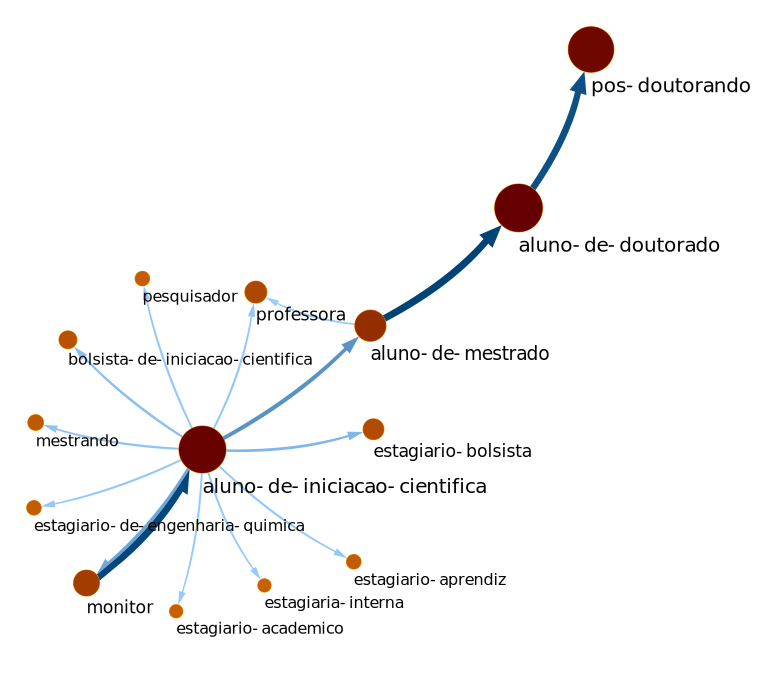
\includegraphics[width=0.5\linewidth]{ex-sobreposicao-aluno-iniciacao2.pdf}
        \label{fig:ex-sobreposicao-ciencia}
    }
    \subfloat[][Recursos Humanos] {
        \includegraphics[width=0.5\linewidth]{ex-sobreposicao-recursos-humanos.pdf}
        \label{fig:ex-sobreposicao-recursos-humanos}
    }
    \\    
    \subfloat[][Ambiental] {
        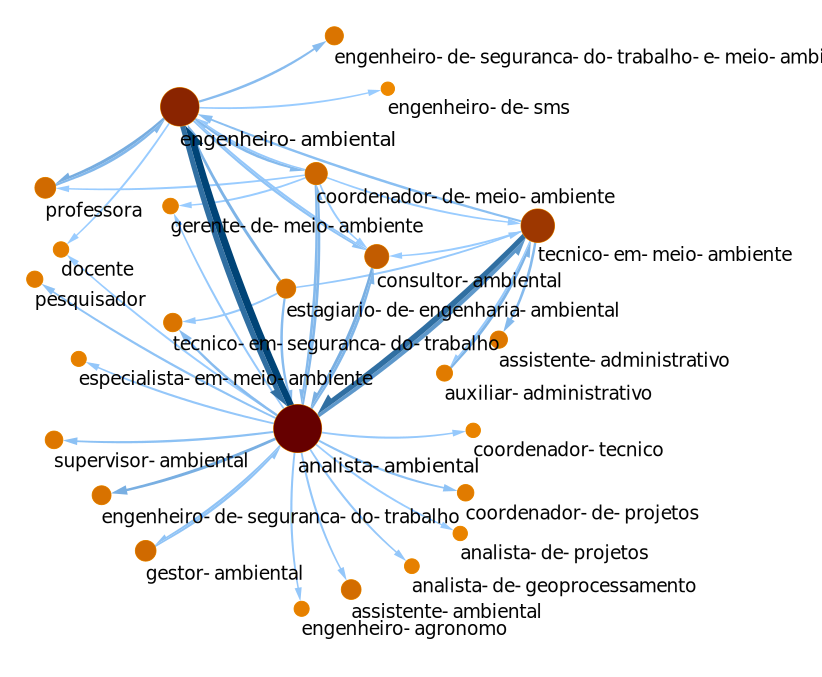
\includegraphics[width=0.5\linewidth]{ex-sobreposicao-analista-ambiental.pdf}
        \label{fig:ex-sobreposicao-analista-ambiental}
    }
    \caption{Três exemplos de ilhas ocupacionais. O tamanho e a cor do nó estão relacionados ao fluxo de profissionais que passa por ele, quanto maior e mais escuro o nó, maior o fluxo. Da mesma forma, a espessura e a cor das conexões está relacionada ao fluxo de profissionais entre uma ocupação e outra. O polos ocupacionais são identificados pelo volume de pessoas transitando por eles e pela sua alta conectividade (visualmente os nós maiores e mais centrais). Para facilitar a visualização, nas Figuras~\ref{fig:ex-sobreposicao-recursos-humanos} e~\ref{fig:ex-sobreposicao-analista-ambiental}, apenas as conexões e nós de maior fluxo são apresentados. A Figura~\ref{fig:ex-sobreposicao-ciencia}, no entanto, mostra a ilha completa.}
    \label{fig:ex-ilhas-ocupacionais}
\end{figure}

%===================================
\section{CONCLUSÕES E PERSPECTIVAS FUTURAS} \label{sec:conclusoes}
%===================================

Esse trabalho reúne os conceitos fronteiras de carreira de \citeonline{Gunz2007-hr}, os trabalhos de Ciência de Redes sobre detecção de comunidades por fluxo baseados em \cite{Rosvall2009-sd} e os dados de um dos maiores sites brasileiros de carreira~\cite{VAGAS_Tecnologia2014-yv} para contribuir na compreensão da movimentação profissional.

A rede profissional possui \textit{hubs}, o que fornece indícios de que carreiras menos regulares são comuns, como advogam as Carreiras sem Fronteiras e Carreiras Proteanas. Ao mesmo tempo a presença de muitos pequenos ego-grafos e ilhas ocupacionais diminutas sugerem que há alternativas para essas teorias.

A Equação de Mapa~\cite{Rosvall2009-sd} foi aplicada usando o software Infomap~\cite{Edler2012-hh} para identificar as fronteiras de carreiras, gerando \textit{ilhas ocupacionais}, que são conjuntos de ocupações em que a movimentação interna é significativamente mais frequente do que movimentações para outras \textit{ilhas}. O termo foi introduzido para facilitar a discussão e como uma analogia ao conceito sugerido por~\cite{Abbott1995-ft} em que a fronteira define o grupo, ao invés do grupo definir a fronteira. Essa abordagem usa a diferença entre os grupos para defini-los ao invés de alguma característica intrínseca. 

A análise da assortatividade das ilhas mostrou que sua topologia tende ao formato estrelado ou de eixo e raios, o que motivou a introdução do termo \textit{polos ocupacionais} para identificar ocupações que dão coesão à ilha. Alguns exemplos emblemáticos dão dimensão aos dois conceitos introduzidos nesse trabalho.

Conclui-se na expectativa que esse trabalho contribua para a compreensão das transições profissionais, no entanto, é preciso reconhecer as limitações dessa proposta e as questões que permanecem abertas.

Os aspectos sociais e psicológicos das fronteiras de carreira não foram abordados e são eles quem podem responder a perguntas como \enquote{por que as fronteiras estão onde estão?} e \enquote{por que as ilhas possuem essa topologia?}. Espera-se que o conteúdo apresentado contribua de maneira quantitativa em discussões sociais e psicológicas sobre movimentação profissional.

Outros trabalhos podem aprofundar a questão da dinâmica da rede, focando em modelos que possam predizer os efeitos esperados quando uma ocupação ganha ou perde atratividade, ou quando um fluxo é incentivado ou estrangulado. Esse trabalho ensaia um começo tímido nessa direção ao propor o conceito de polos ocupacionais e identificar sua importância nas ilhas de ocupações.

Outra linha de pesquisa atrativa está em comparar o MCar com redes aleatórias geradas a partir de características similares à da rede real, procurando identificar quais delas resultam em observações comparáveis. Essas características indicam possíveis explicações para os comportamentos encontrados a partir de uma abordagem puramente estatística~\cite{Barabasi2016-rn}.

O MCar é uma fonte considerável de informação sobre o mercado de trabalho brasileiro. Outras pesquisas sobre profissões e carreira, em especial utilizando técnicas de Ciência de Redes, como \textit{motifs}, podem contribuir para uma melhor compreensão da movimentação profissional.

\FloatBarrier % 'Floats' (imagens) não devem passar daqui!

\def\refname{REFERÊNCIAS BIBLIOGRÁFICAS}
\bibliography{main}
\addcontentsline{toc}{section}{REFERÊNCIAS BIBLIOGRÁFICAS}
\bibliographystyle{abnt-alf}

\end{document}
